\chapter{Análise de Cargas}
\label{cap:analise_cargas}

\section{Representação dos carregamentos}
\label{sec:representacao_carregamentos}

A Figura~\ref{fig:forcas_aeronave} apresenta as principais forças e o momento aerodinâmico atuantes na aeronave, enquanto a Figura~\ref{fig:cargas_distribuidas} representa esquematicamente as cargas distribuídas na asa, na empenagem horizontal e ao longo da fuselagem. Esses esquemas ilustram os carregamentos considerados na análise, cujas condições de aplicação são definidas a partir do diagrama V--n e utilizadas no dimensionamento estrutural.

\begin{figure}[H]
    \centering
    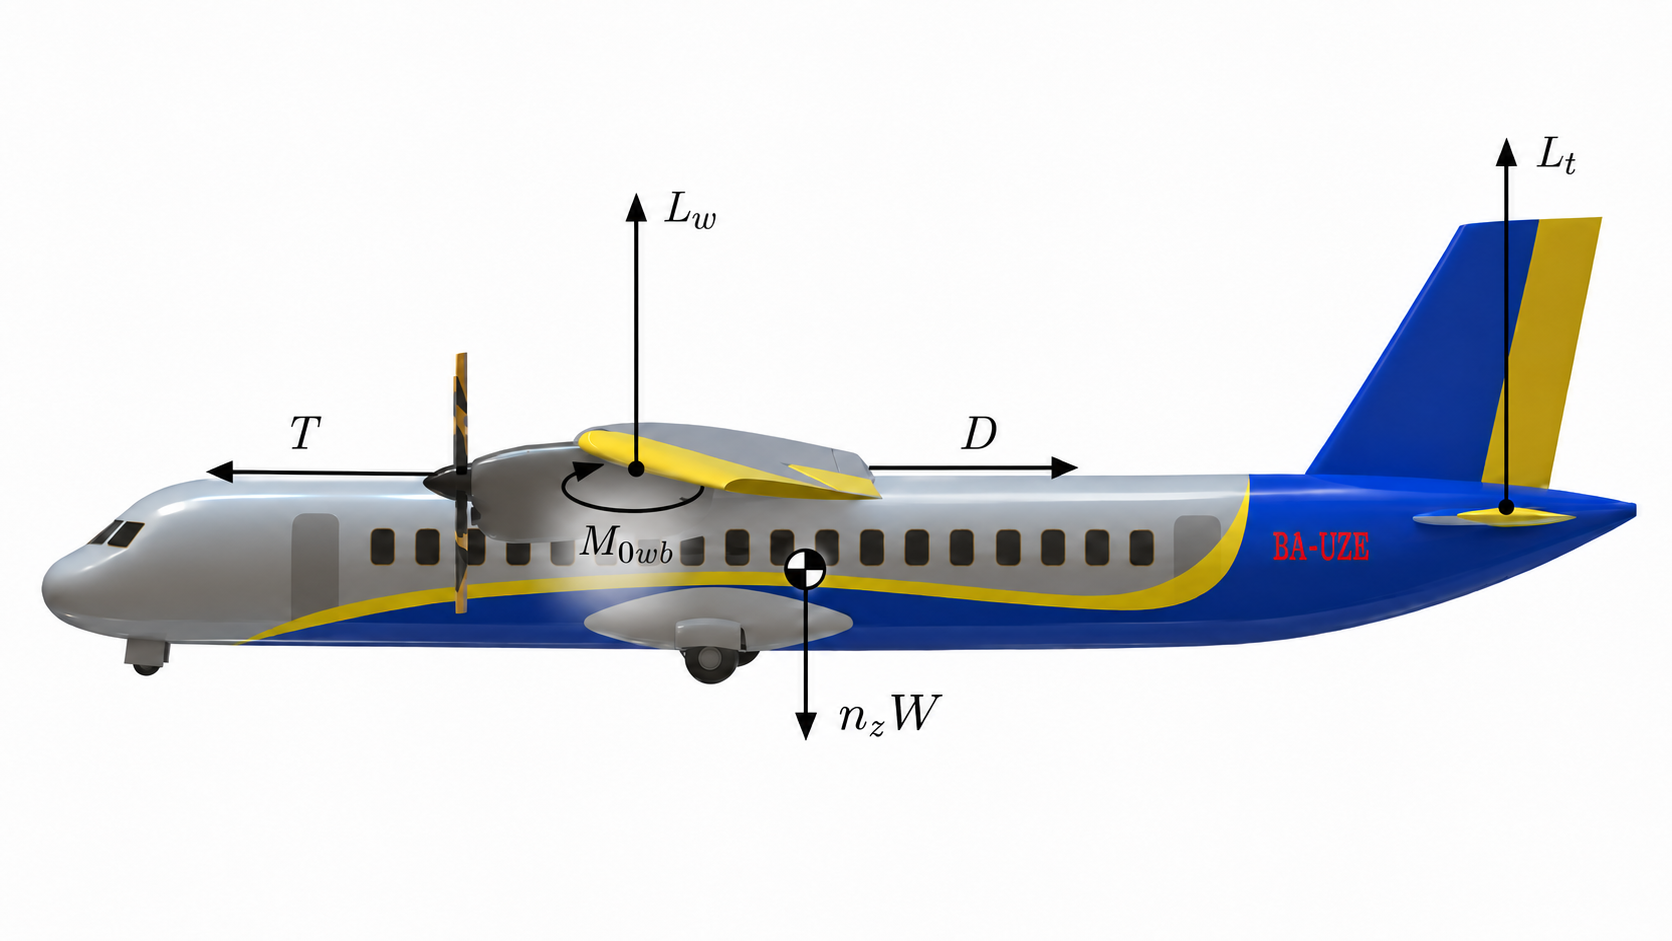
\includegraphics[width=0.85\textwidth]{images/cargas/Diagrama técnico de forças em aeronave.png}
    \caption{Principais forças e momento aerodinâmico atuantes na aeronave.}
    \label{fig:forcas_aeronave}
\end{figure}

\begin{figure}[H]
    \centering
    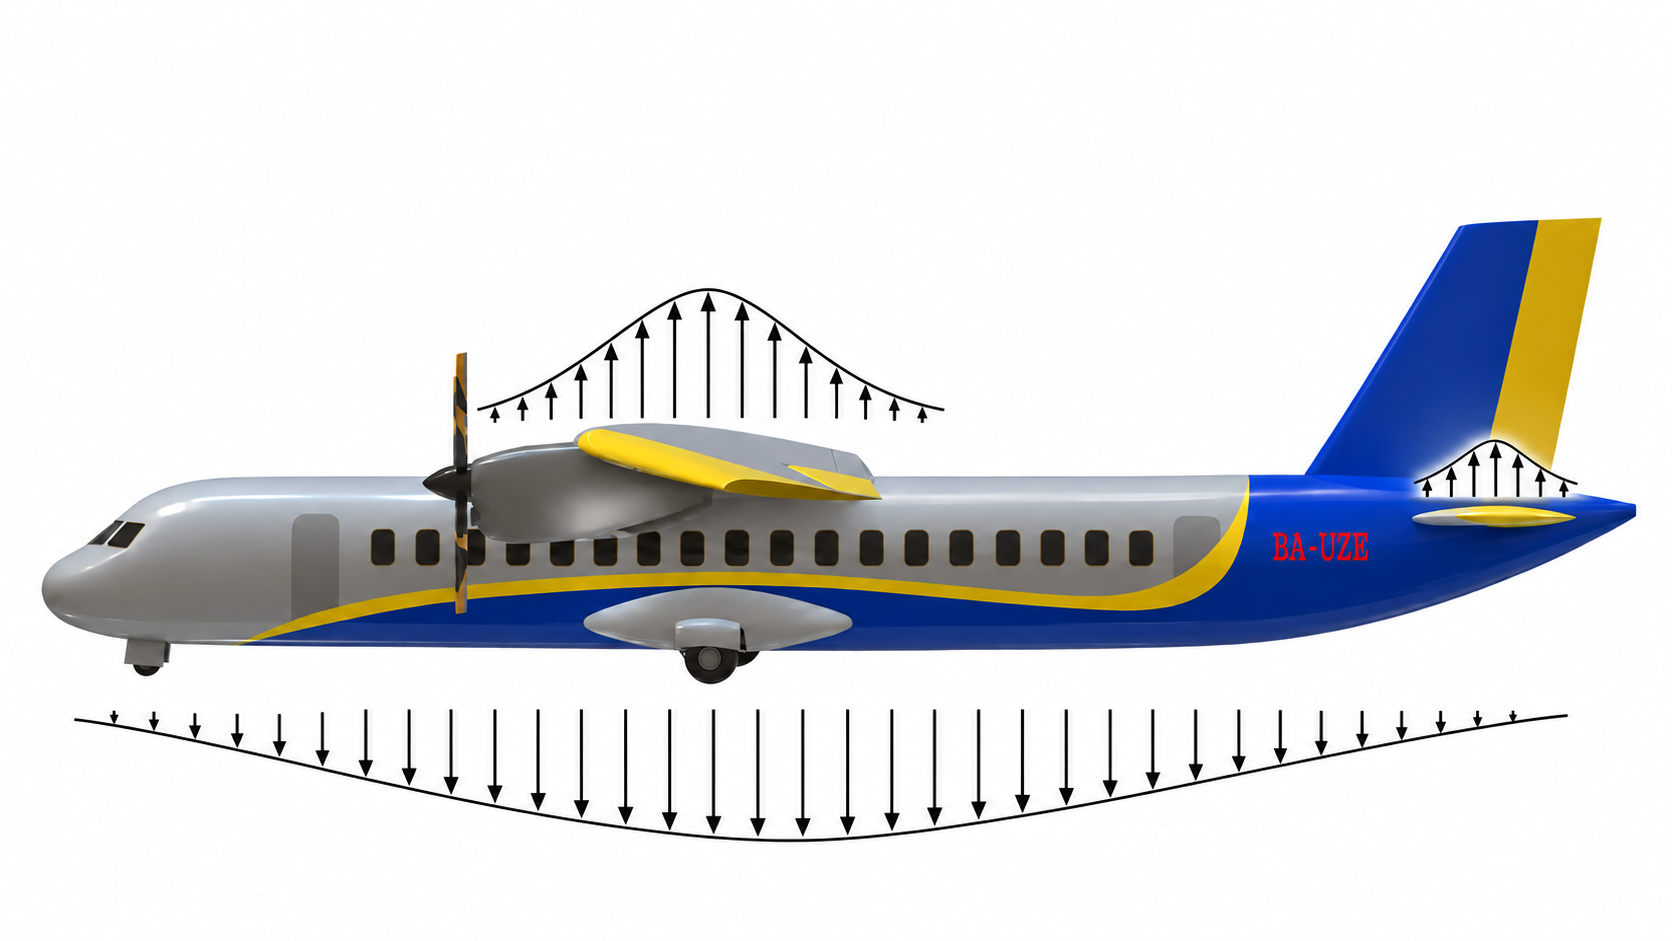
\includegraphics[width=0.85\textwidth]{images/cargas/Aeronave com diagramas de cargas distribuídas.png}
    \caption{Distribuição esquemática de cargas na aeronave.}
    \label{fig:cargas_distribuidas}
\end{figure}

\section{Diagrama V--n}
\label{sec:cargas_vn}

O diagrama V-n foi construído conforme o 14 CFR Part 25. As velocidades de projeto, em velocidade
equivalente, foram obtidas pelo \S 25.335 a partir do MTOW, da área alar $S = 74{,}1$~m$^2$ e dos
$C_{L_{max}}$ de cada configuração (1,50 limpo; 1,88 com flap de 10°; 2,69 com flap de 40°). Como os
valores de $V_C$ e $V_D$ adotados anteriormente eram inferiores aos mínimos da norma, foram
utilizados $V_C = 230$~kt ($V_C \geq V_B + 1{,}32\,U_{ref}$) e $V_D = 288$~kt ($V_C/V_D \leq 0{,}8$).
Os fatores de carga limite de manobra são $+2{,}5$ e $-1{,}0$ com flaps recolhidos (\S 25.337) e
$+2{,}0$ com flaps baixados (\S 25.345). As cargas de rajada foram estimadas pelo modelo quase-estático
de Pratt, com o fator de alívio $K_g$ do \S 25.335(d) e a velocidade de rajada de projeto do
\S 25.341(a) ($U_{de} = 41{,}1$~ft/s entre $V_B$ e $V_C$ ao nível do mar e 25~ft/s com flaps). As
Figuras~\ref{fig:vn_manobra} a \ref{fig:vn_projeto_20k} apresentam, respectivamente, o envelope de
manobra com flaps recolhidos e baixados, as linhas de rajada e o envelope de projeto resultante ao nível
do mar e a 20\,000~ft. Em todas as condições o envelope de manobra é o crítico.

\begin{figure}[H]
    \centering
    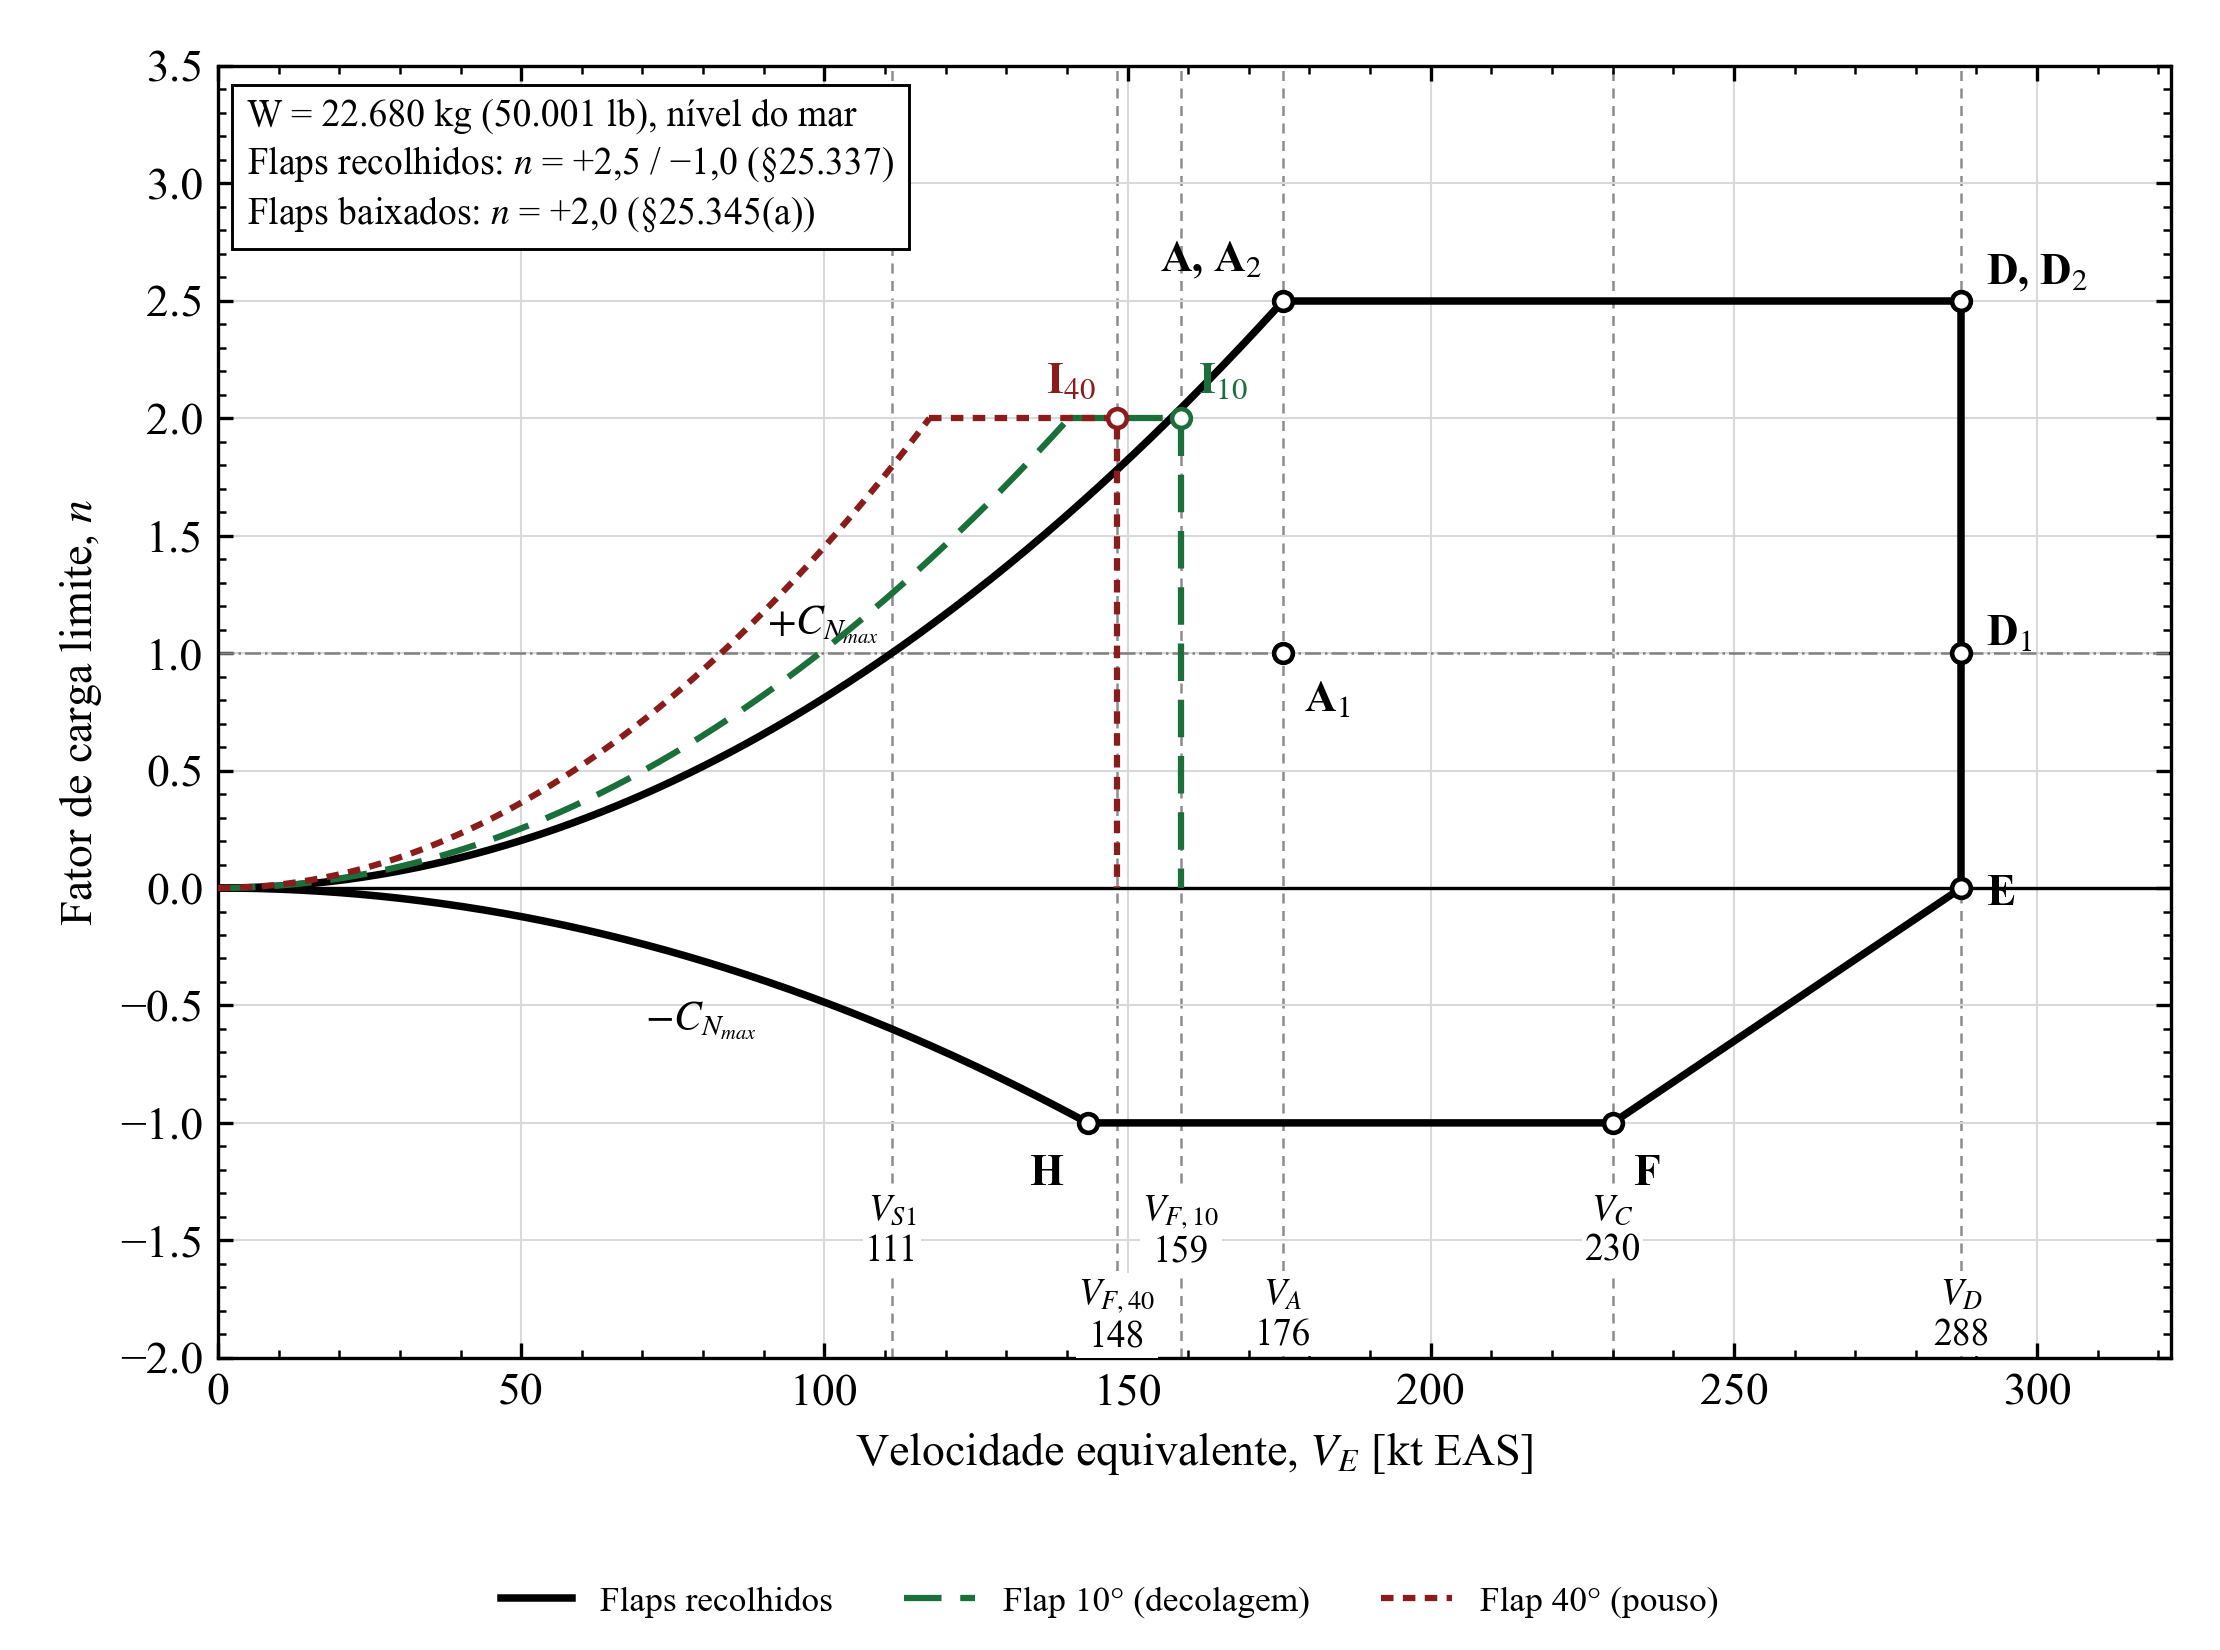
\includegraphics[width=0.95\linewidth]{images/cargas/vn_manobra_sl.png}
    \caption{Diagrama V-n de manobra com flaps recolhidos e baixados (10° e 40°), MTOW, nível do mar.}
    \label{fig:vn_manobra}
\end{figure}

\begin{figure}[H]
    \centering
    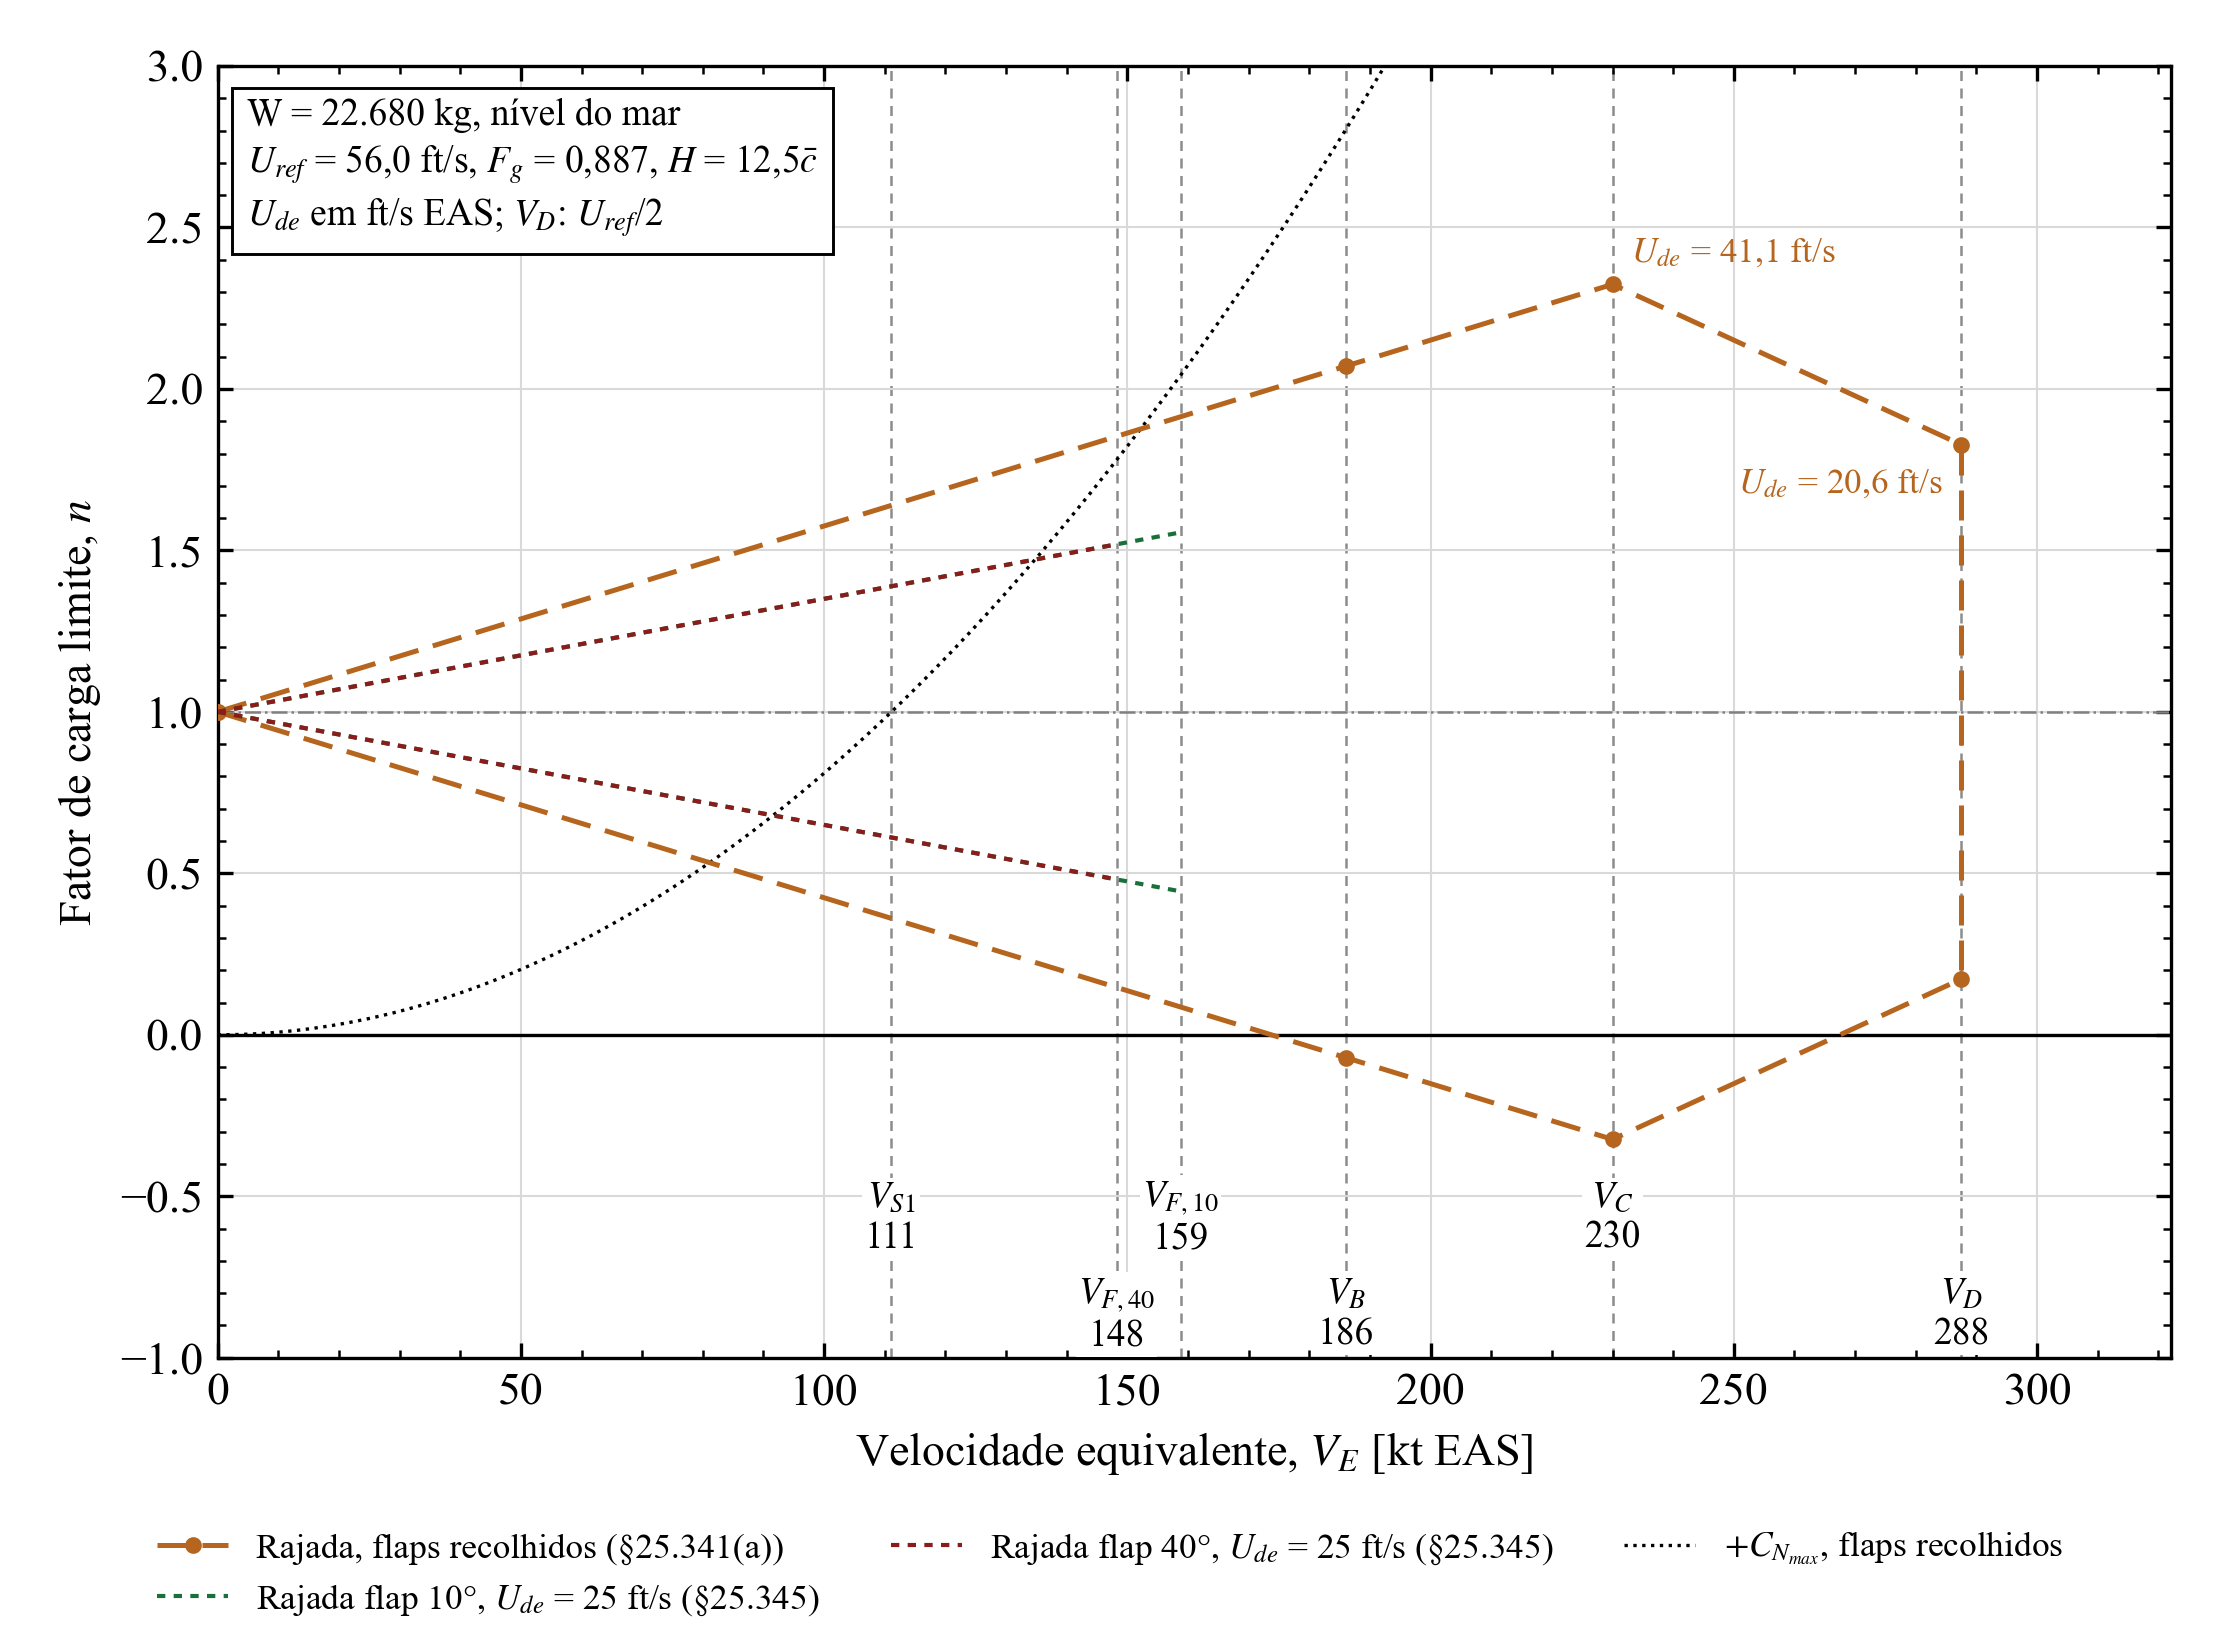
\includegraphics[width=0.95\linewidth]{images/cargas/vn_rajada_sl.png}
    \caption{Diagrama V-n de rajada com flaps recolhidos e baixados (10° e 40°), MTOW, nível do mar.}
    \label{fig:vn_rajada}
\end{figure}

\begin{figure}[H]
    \centering
    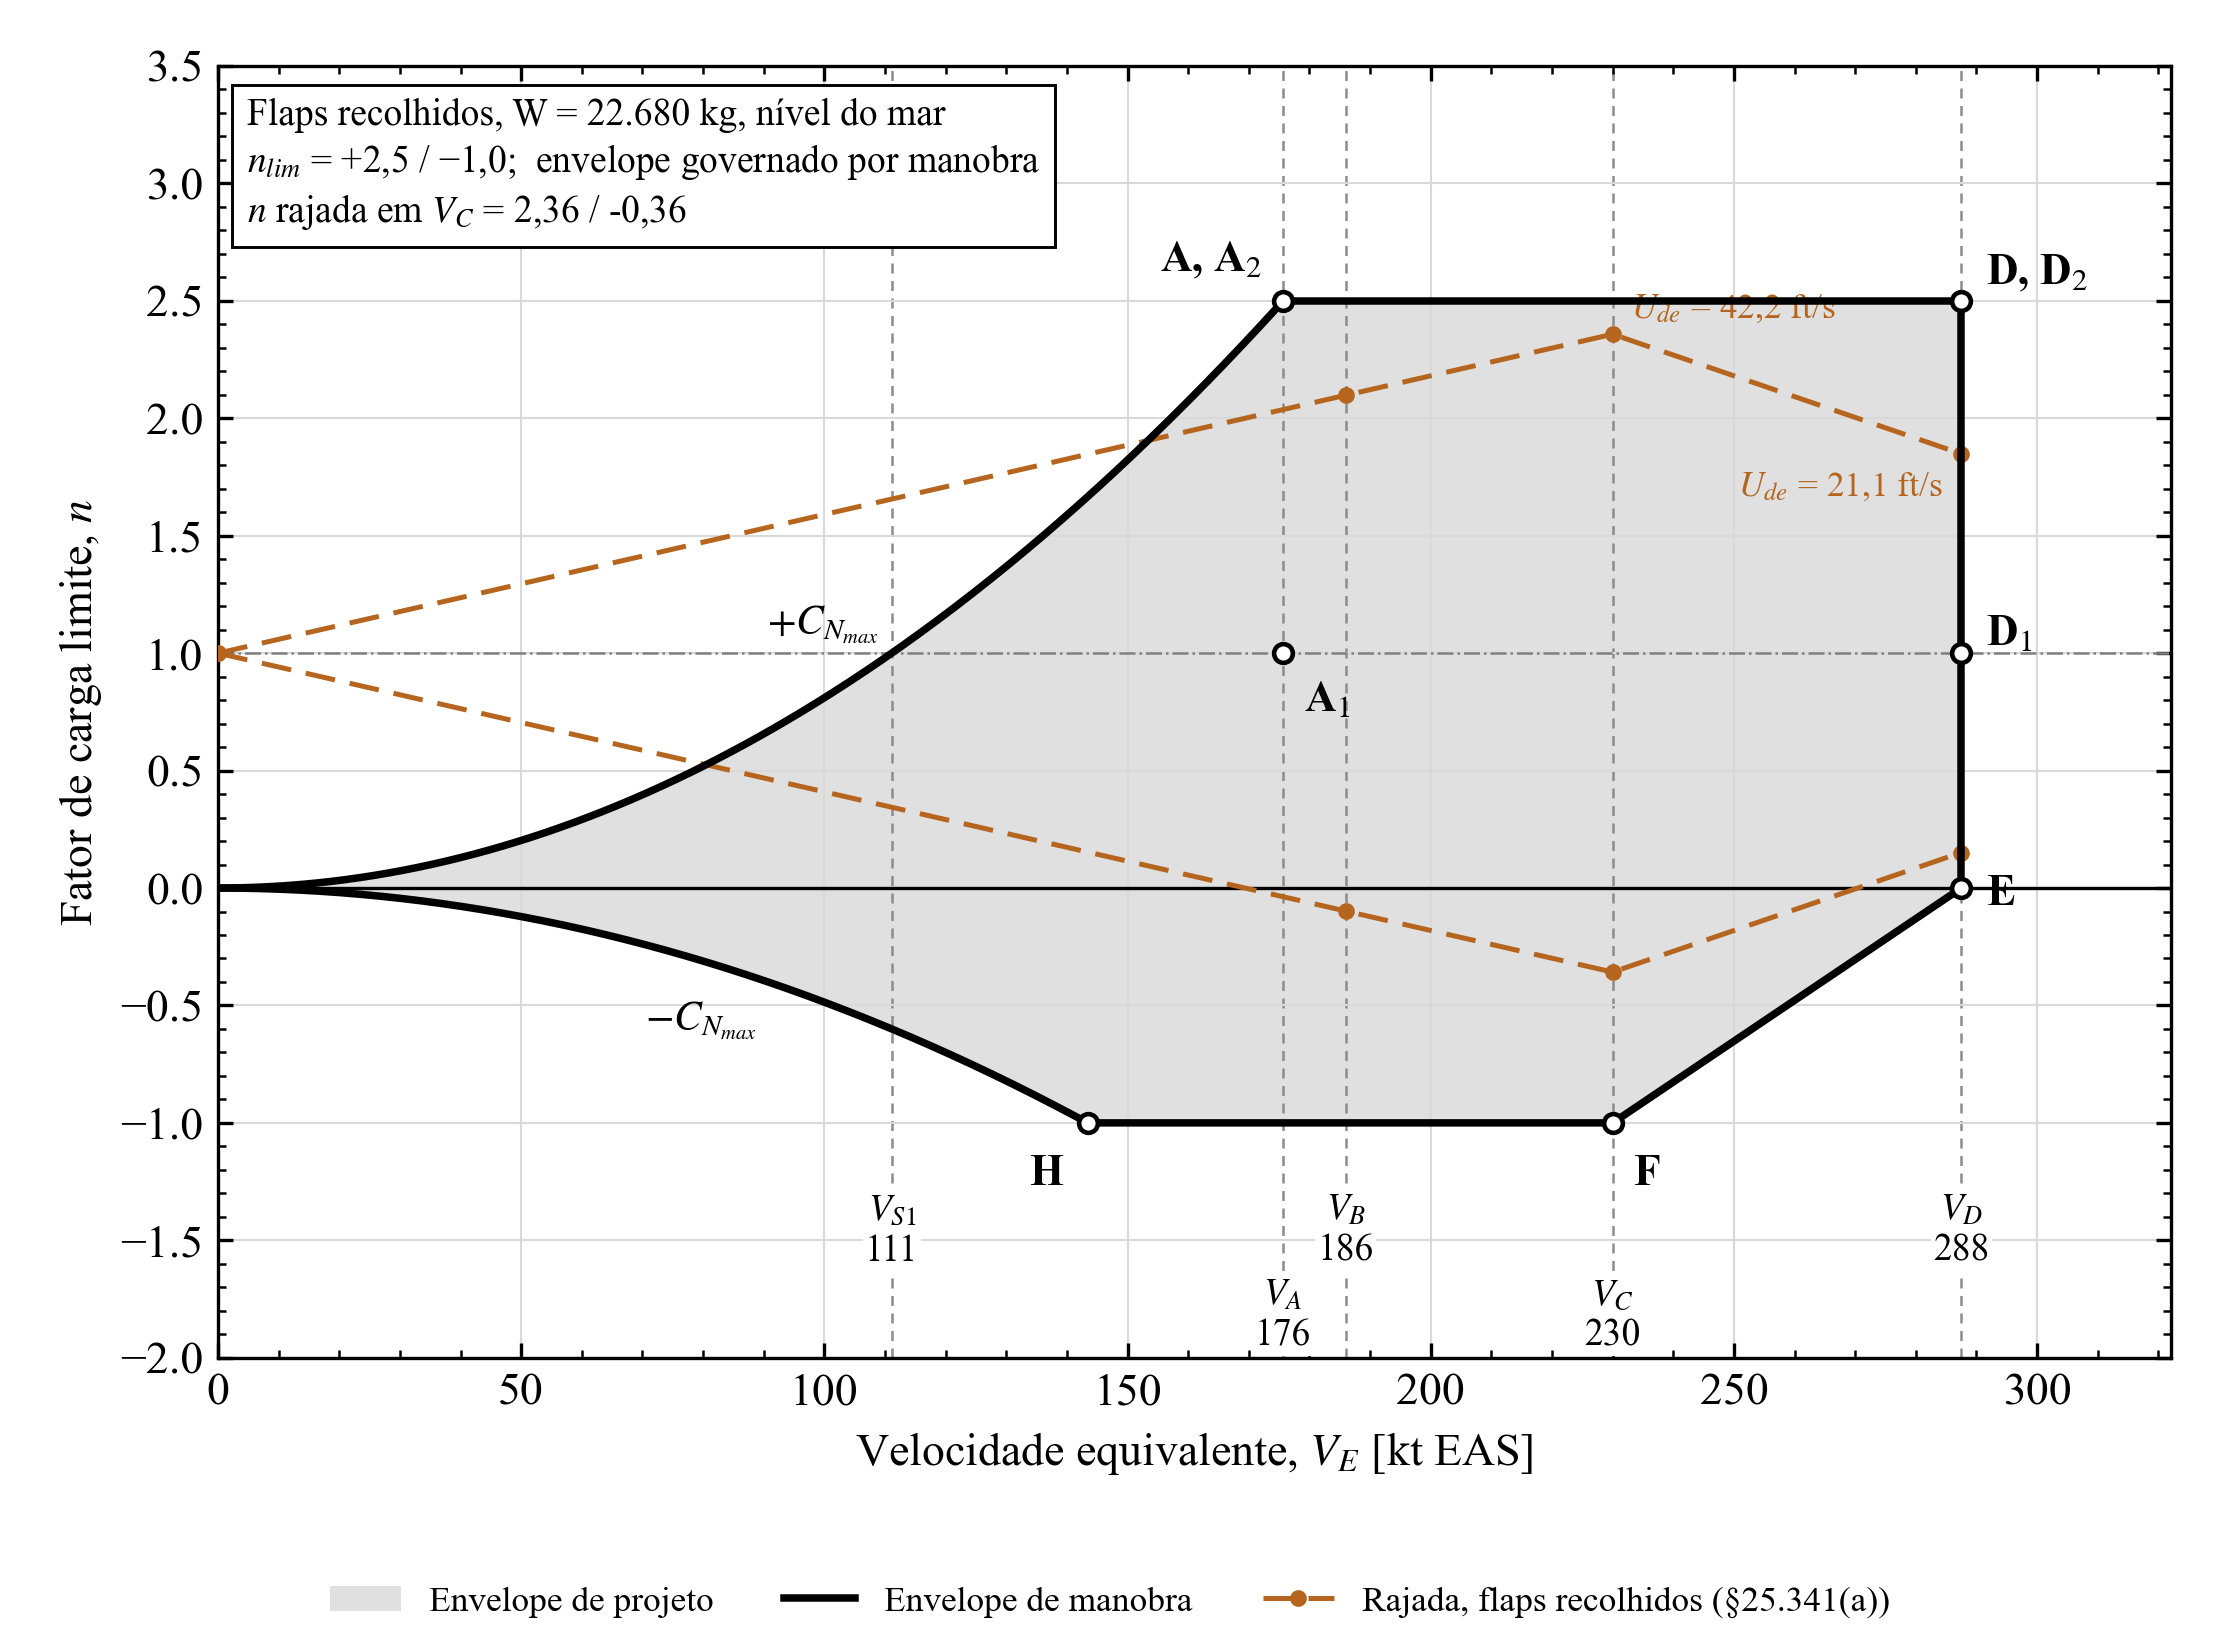
\includegraphics[width=0.95\linewidth]{images/cargas/vn_projeto.png}
    \caption{Envelope de projeto (manobra e rajada) com flaps recolhidos, MTOW, nível do mar.}
    \label{fig:vn_projeto_sl}
\end{figure}

\begin{figure}[H]
    \centering
    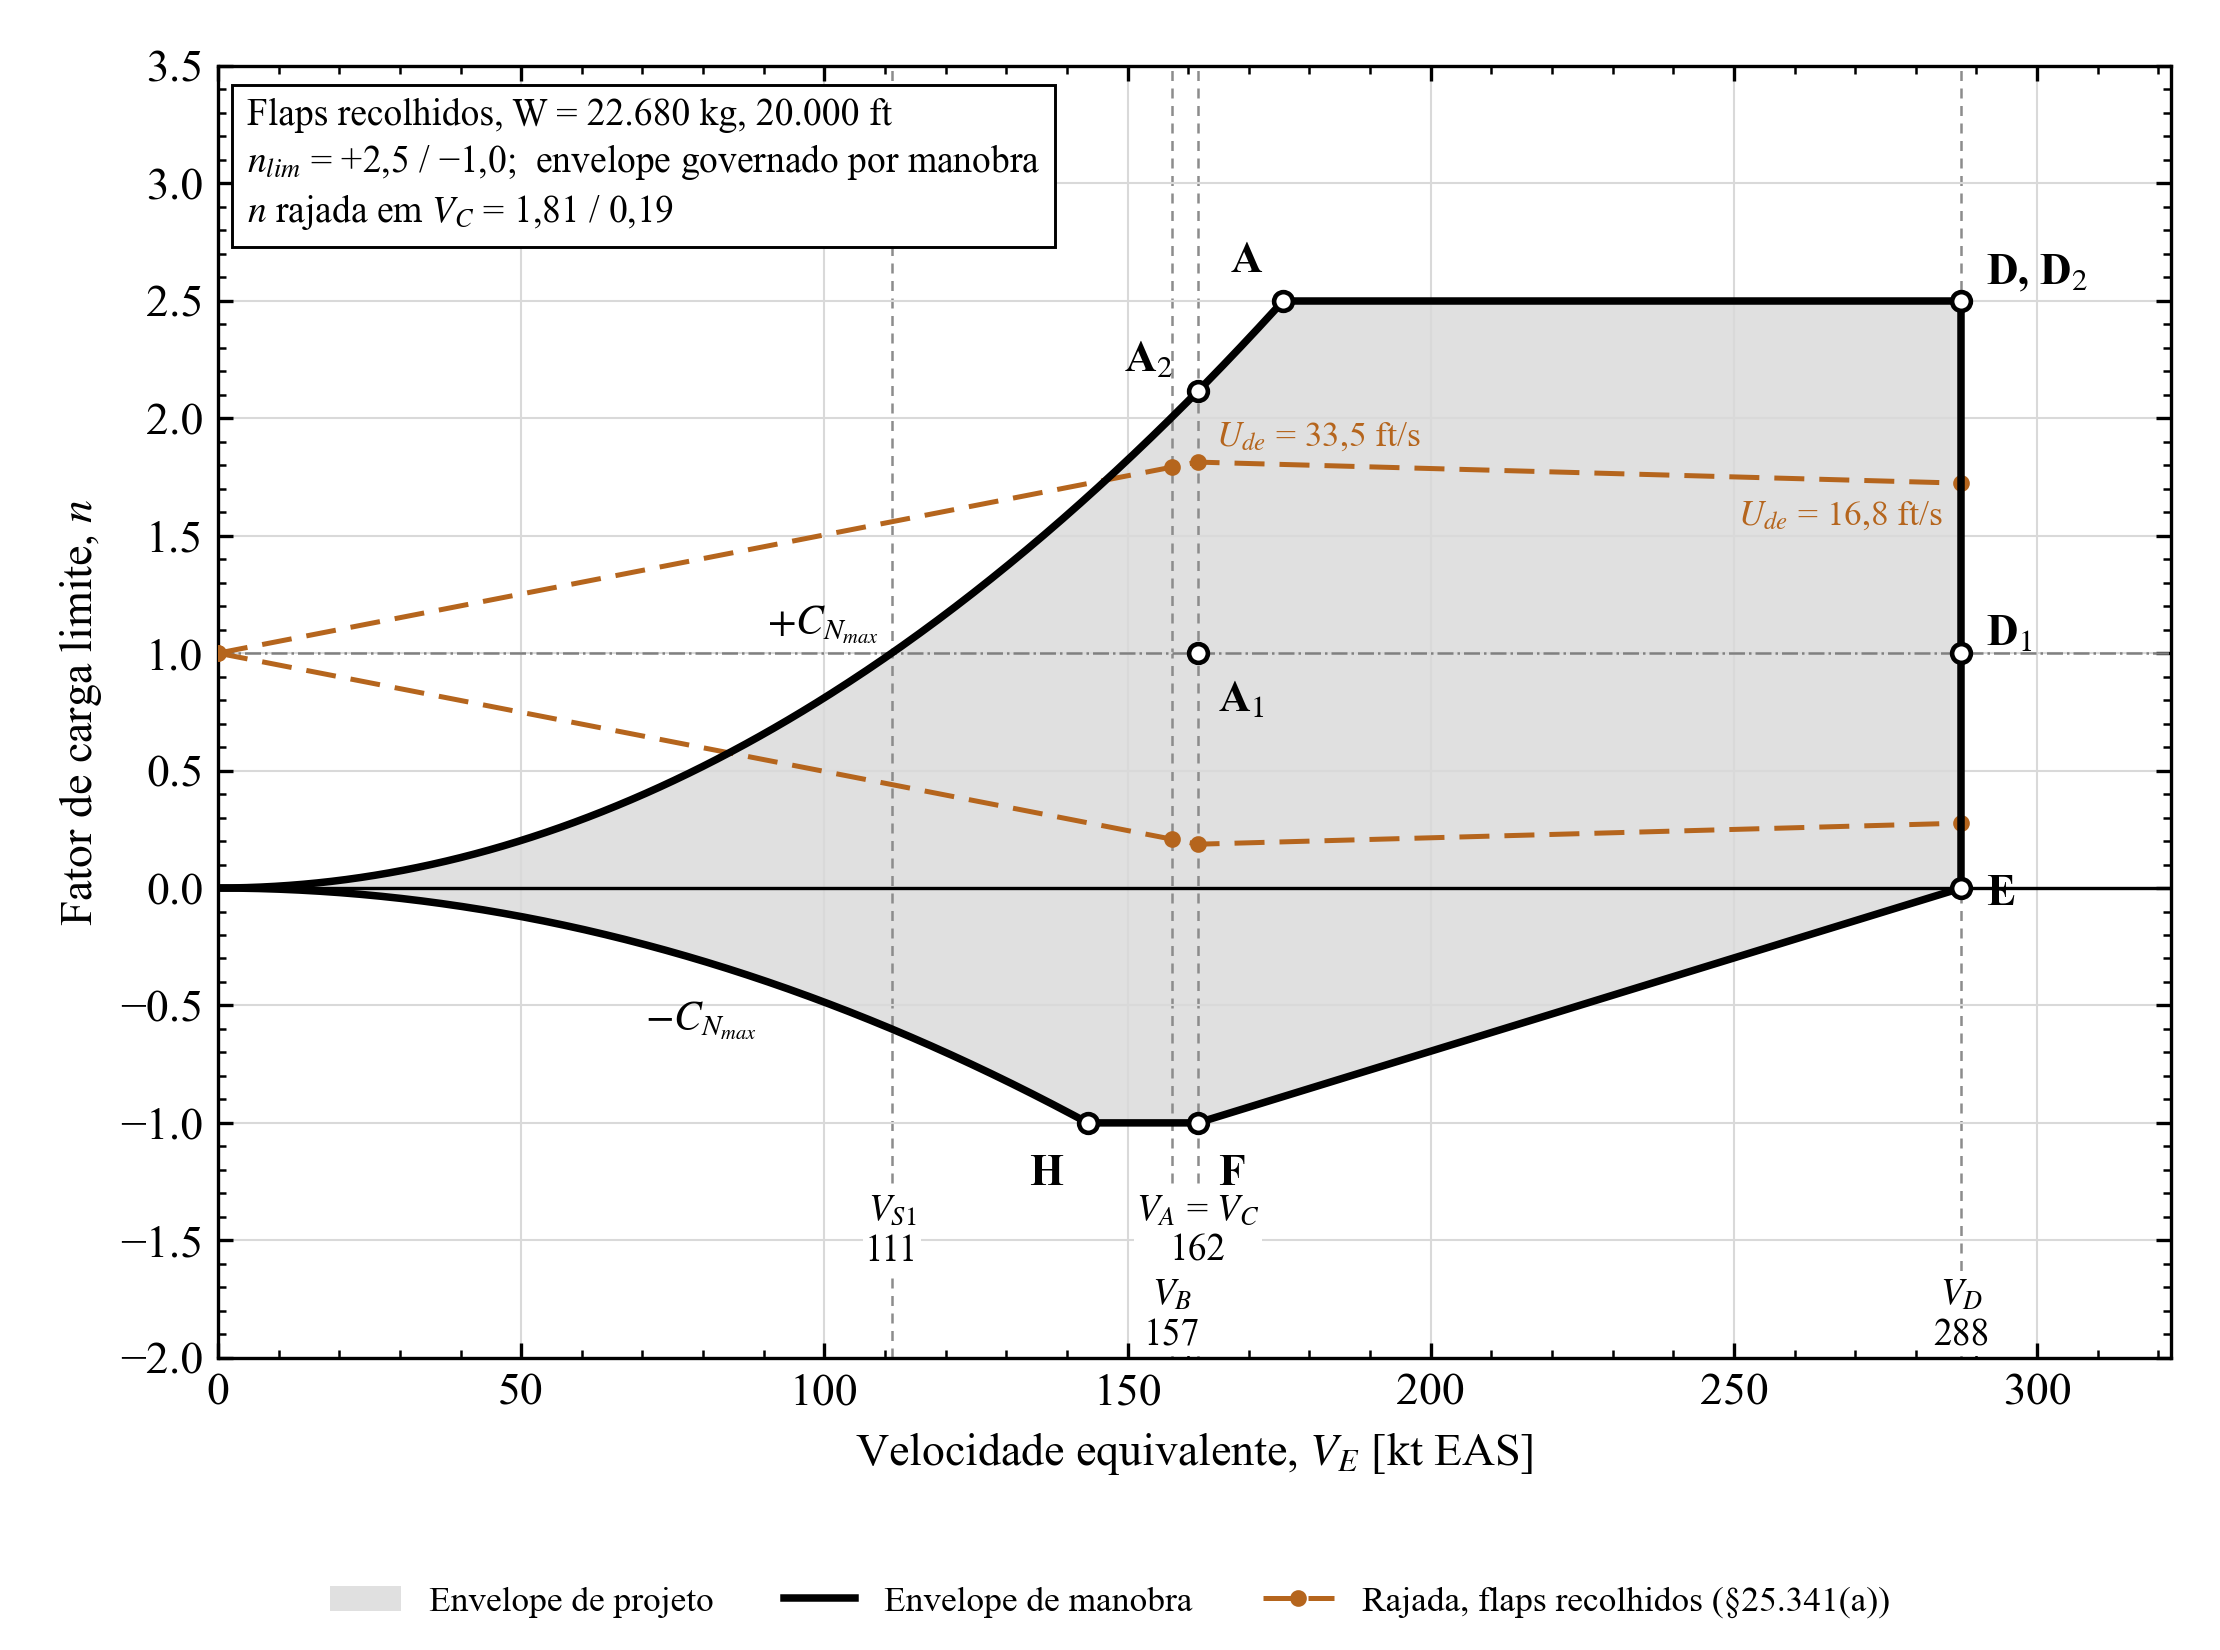
\includegraphics[width=0.95\linewidth]{images/cargas/vn_projeto_20000ft.png}
    \caption{Envelope de projeto (manobra e rajada) com flaps recolhidos, MTOW, 20.000 ft.}
    \label{fig:vn_projeto_20k}
\end{figure}




\section{Cargas na Asa}
\label{sec:cargas_asa}

A análise de cargas na asa considerou as condições de manobra e os pontos do envelope de rajada. As cargas aerodinâmicas foram determinadas para cada condição e distribuídas ao longo da envergadura pelo método de Stender, permitindo o cálculo dos esforços internos correspondentes.

\subsection*{Manobra e Balanceamento Longitudinal}

Para as condições simétricas de manobra, a sustentação da asa foi determinada a partir do equilíbrio longitudinal da aeronave, considerando as forças aerodinâmicas da asa e da EH, o peso e o momento aerodinâmico do conjunto asa--fuselagem, conforme representado na \autoref{fig:cargas_dcl_balanceamento}. Dessa forma, a carga de balanceamento da EH foi considerada na determinação dos carregamentos da asa, conforme o \S~25.331 do 14 CFR Part 25. Os momentos produzidos pelas forças de arrasto e tração foram desconsiderados no equilíbrio longitudinal.

\begin{figure}[H]
    \centering
    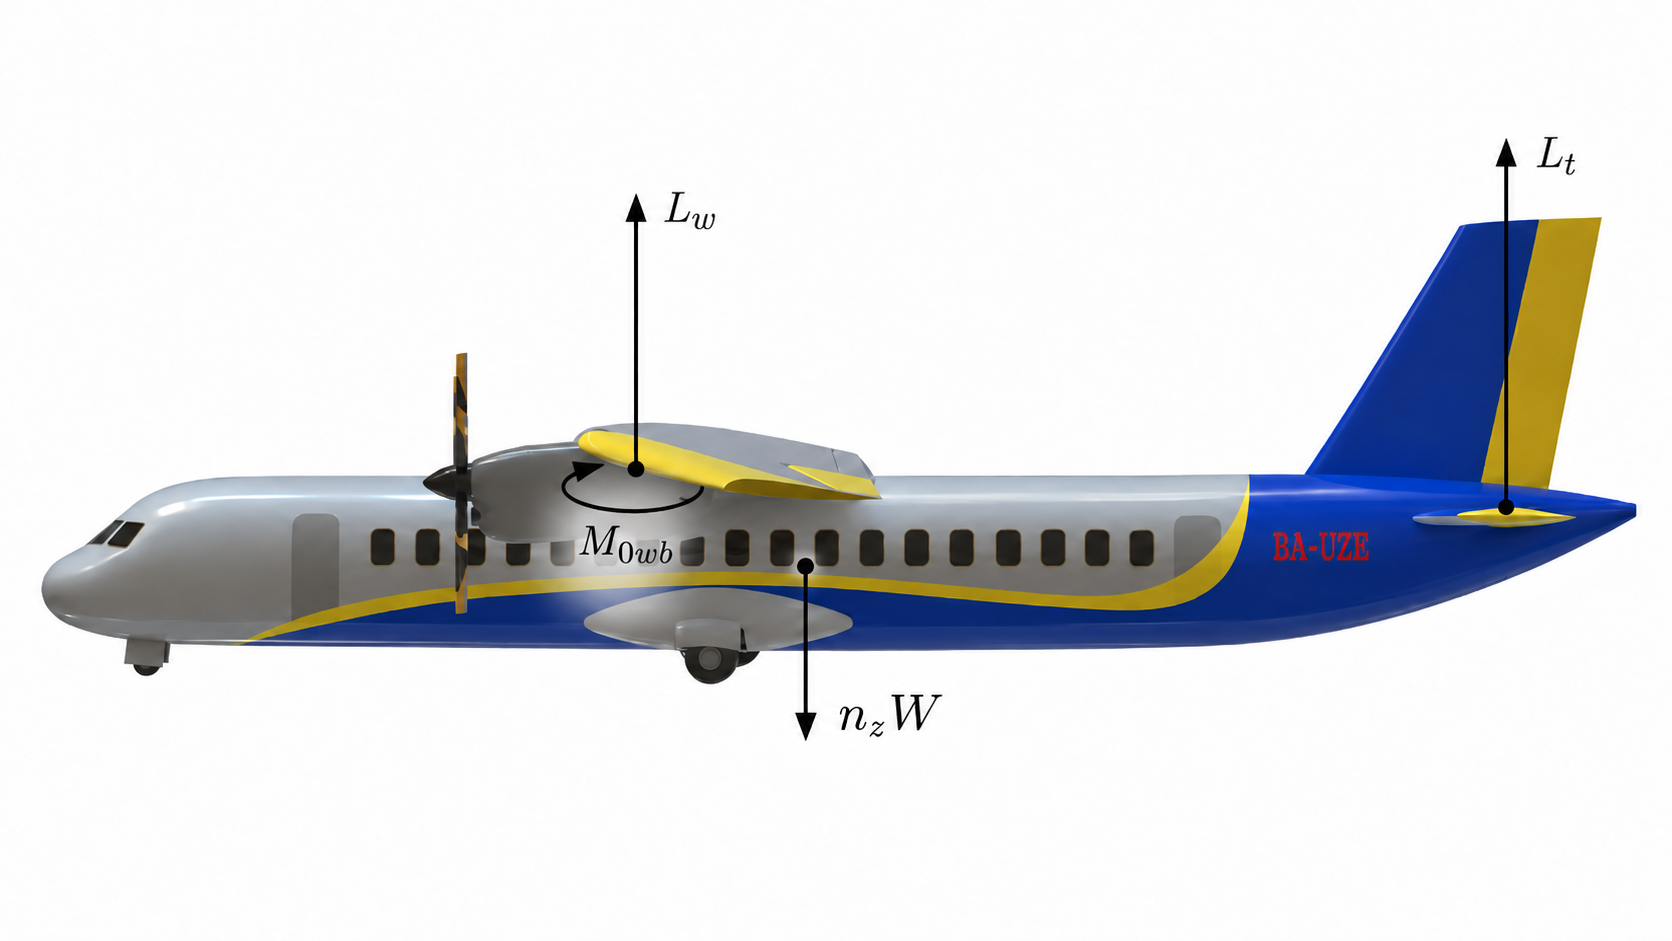
\includegraphics[width=0.85\linewidth]{images/cargas/DCL_cargas.png}
    \caption{Diagrama de corpo livre do equilíbrio longitudinal.}
    \label{fig:cargas_dcl_balanceamento}
\end{figure}

A carga resultante na asa foi calculada por:
\begin{equation}
    L_w=-\frac{\rho_0 S_w\bar{c}C_{M_0}}{2\bar{l}_t}V_{\mathrm{EAS}}^2
    +\frac{W\left[\bar{l}_t-(h_{CG}-h_0)\bar{c}\right]}{\bar{l}_t}\,n_z,
    \label{eq:cargas_Lw}
\end{equation}

A Equação~\ref{eq:cargas_Lw} foi avaliada para as combinações de velocidade, fator de carga e posição do CG consideradas nos diagramas $V$--$n$.

\subsection*{Rajada}

Para os pontos do envelope de rajada, os fatores de carga obtidos conforme a metodologia adotada com referência ao \S~25.341 do 14 CFR Part 25 foram aplicados à Equação~\ref{eq:cargas_Lw}.

\subsection*{Arrasto, Momento Aerodinâmico e Distribuição}

O arrasto de perfil foi estimado a partir da sustentação local, obtida pela distribuição de Stender, e das polares bidimensionais dos perfis utilizados. Os coeficientes de momento aerodinâmico também foram obtidos dessas polares e considerados constantes para cada perfil, com o momento referido a $25\%$ da corda local.

Para as regiões da asa encobertas pela fuselagem, as parcelas de sustentação, arrasto e momento aerodinâmico foram redistribuídas sobre os trechos expostos, preservando-se as resultantes dos carregamentos.

As componentes de força foram calculadas pela transformação dos eixos aerodinâmicos para os eixos da aeronave:
\begin{align}
    F_z &= L_w\cos\alpha+D_w\sin\alpha, \\
    F_x &=-L_w\sin\alpha+D_w\cos\alpha.
    \label{eq:cargas_transform_asa}
\end{align}

\subsection*{Resultados}

Os carregamentos distribuídos obtidos pelo método de Stender são apresentados na \autoref{fig:cargas_asa_fz}, na \autoref{fig:cargas_asa_fx} e na \autoref{fig:cargas_asa_ma}.

%% Os gráficos de distribuição abaixo abrangem TODAS as condições de carga da asa.
\begin{figure}[H]
    \centering
    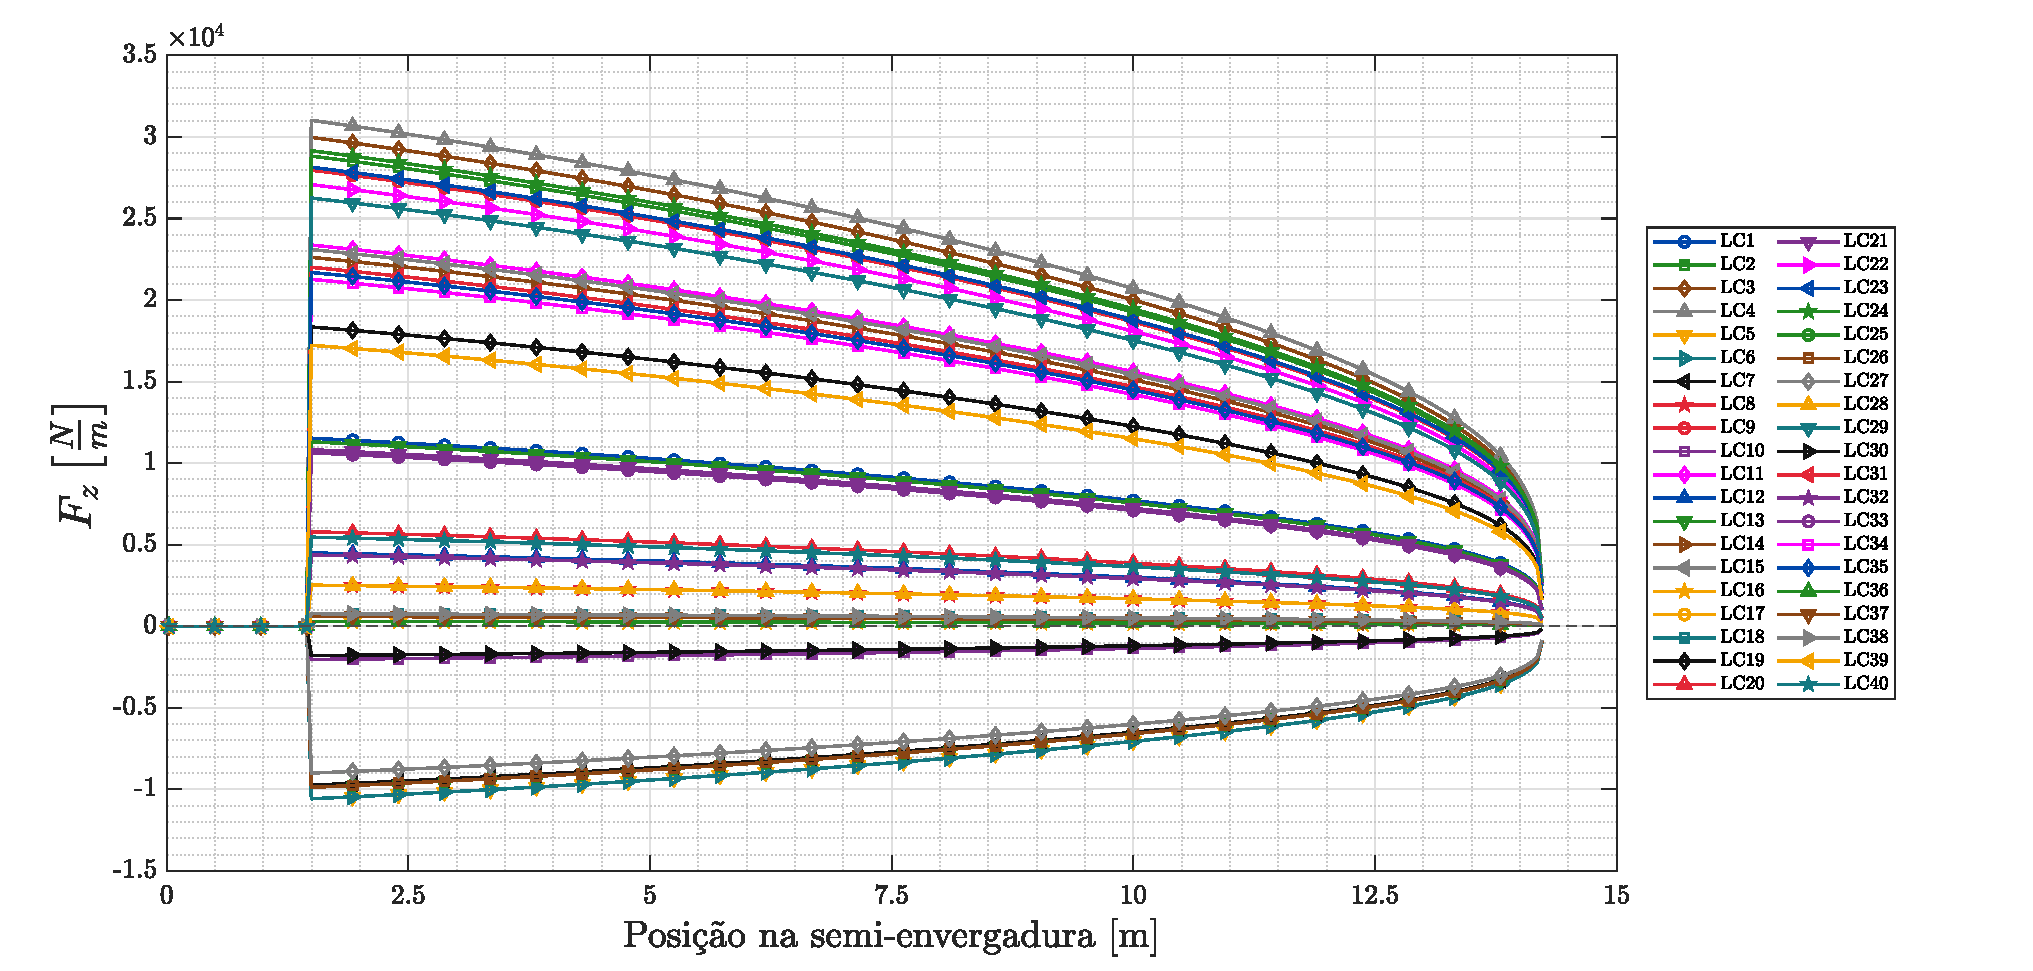
\includegraphics[width=1\linewidth]{images/cargas/wing_Fz.eps}
    \caption{$F_z$ distribuído na asa.}
    \label{fig:cargas_asa_fz}
\end{figure}

\begin{figure}[H]
    \centering
    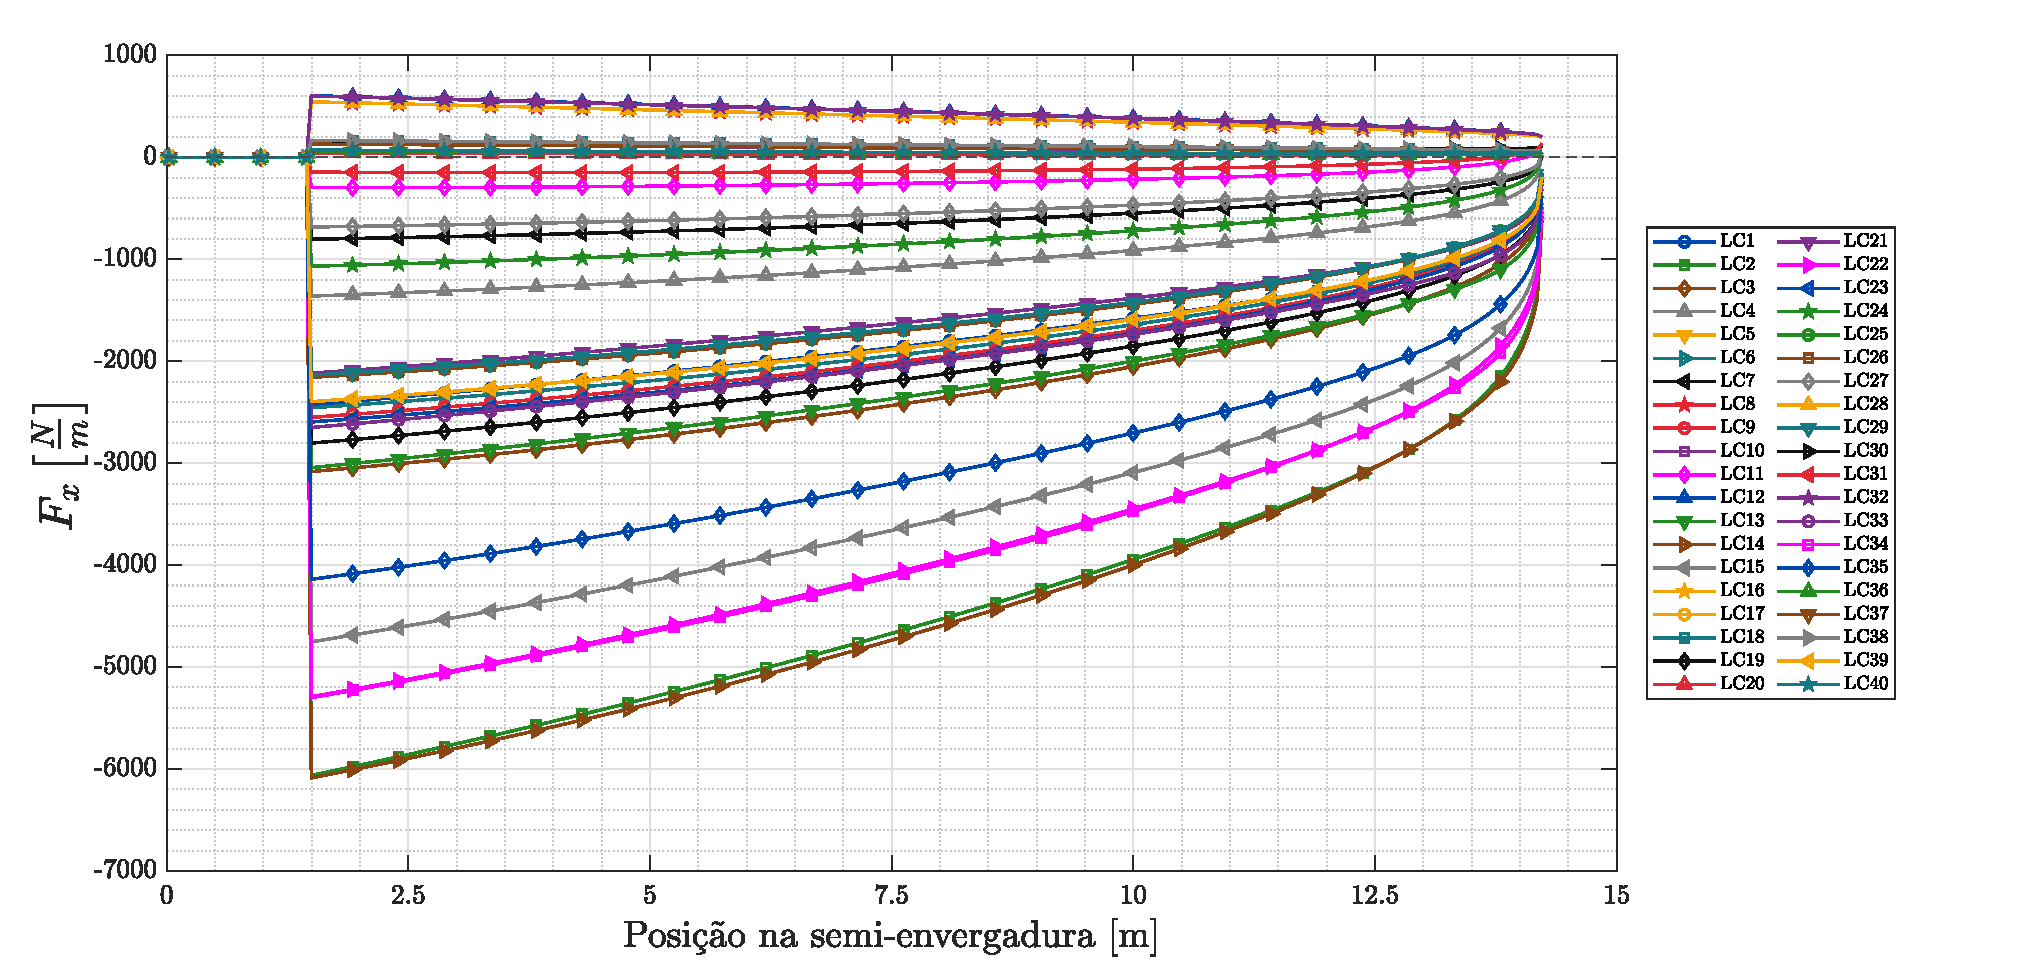
\includegraphics[width=1\linewidth]{images/cargas/wing_Fx.eps}
    \caption{$F_x$ distribuído na asa.}
    \label{fig:cargas_asa_fx}
\end{figure}

\begin{figure}[H]
    \centering
    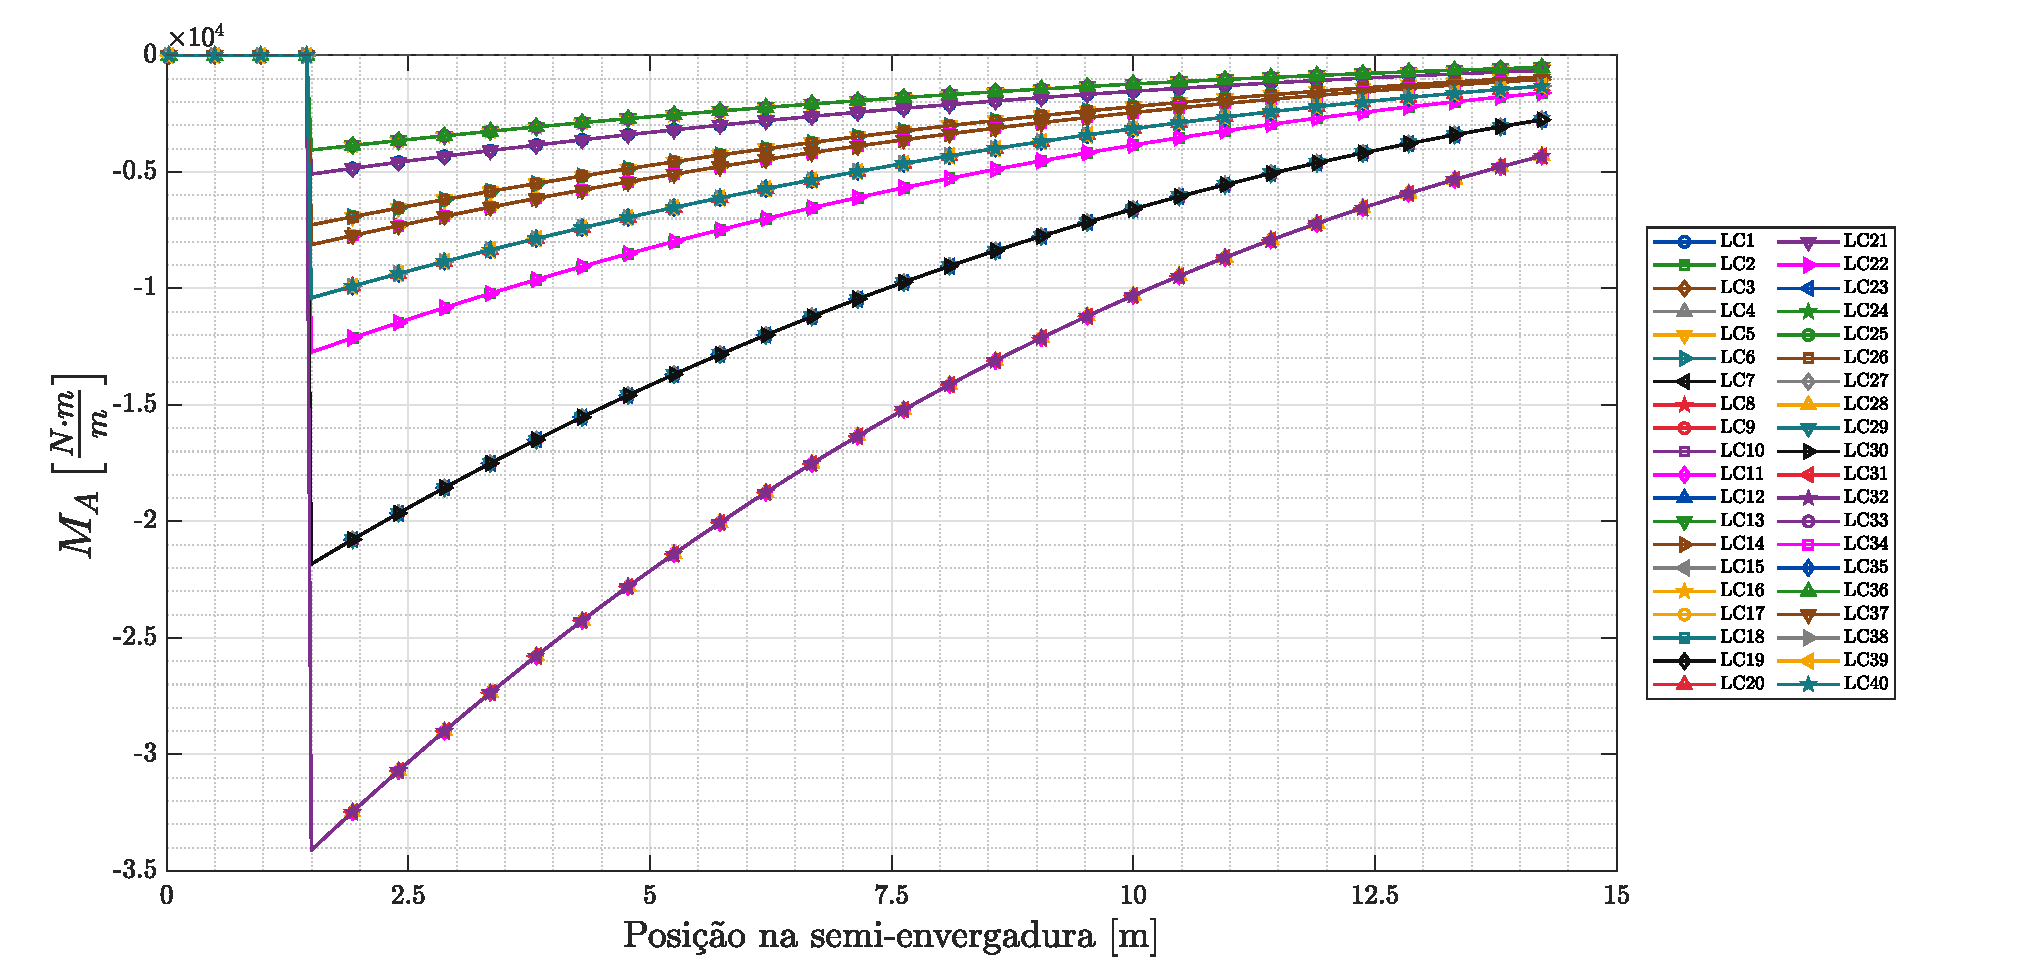
\includegraphics[width=1\linewidth]{images/cargas/wing_MA.eps}
    \caption{$MA$ distribuído na asa.}
    \label{fig:cargas_asa_ma}
\end{figure}

As condições de voo correspondentes aos casos críticos identificados para a asa são resumidas na Tabela~\ref{tab:cargas_criticas_asa}.

\begin{table}[H]
    \centering
    \caption{Condições críticas da asa.}
    \label{tab:cargas_criticas_asa}
    \vspace{1mm}
    \begingroup
    \footnotesize
    \setlength{\tabcolsep}{5pt}
    \renewcommand{\arraystretch}{1.35}
    \begin{tabular}{@{}lccccccc@{}}
        \noalign{\hrule height 0.8pt}
        \textbf{N\textsuperscript{o}} & \textbf{Tipo} & \textbf{14 CFR Part 25} & \textbf{TOW} & \textbf{CG} & \textbf{Flap} & \textbf{Velocidade} & \boldmath$n_z$\\
        \hline
        LC4  & Manobra & \S~25.331 & MTOW & Dianteiro & Recolhido & $V_D$ & $2{,}50$\\
        LC5  & Manobra & \S~25.337 & MTOW & Dianteiro & Recolhido & $V_{S,\mathrm{neg}}$ & $-1{,}00$\\
        LC12 & Rajada  & \S~25.341 & MTOW & Dianteiro & Recolhido & $V_D$ & $0{,}173$\\
        LC14 & Manobra & \S~25.345 & MTOW & Dianteiro & Estendido & $V_A$ & $2{,}00$\\
        LC16 & Manobra & \S~25.345 & MTOW & Dianteiro & Estendido & $V_{SF}$ & $0{,}00$\\
        \noalign{\hrule height 0.8pt}
    \end{tabular}
    \endgroup
\end{table}

Os esforços internos correspondentes às condições críticas são apresentados na \autoref{fig:cargas_asa_crit_fz}, na \autoref{fig:cargas_asa_crit_fx} e na \autoref{fig:cargas_asa_crit_my}.

%% Os gráficos de esforços abaixo incluem SOMENTE as condições críticas.
\begin{figure}[H]
    \centering
    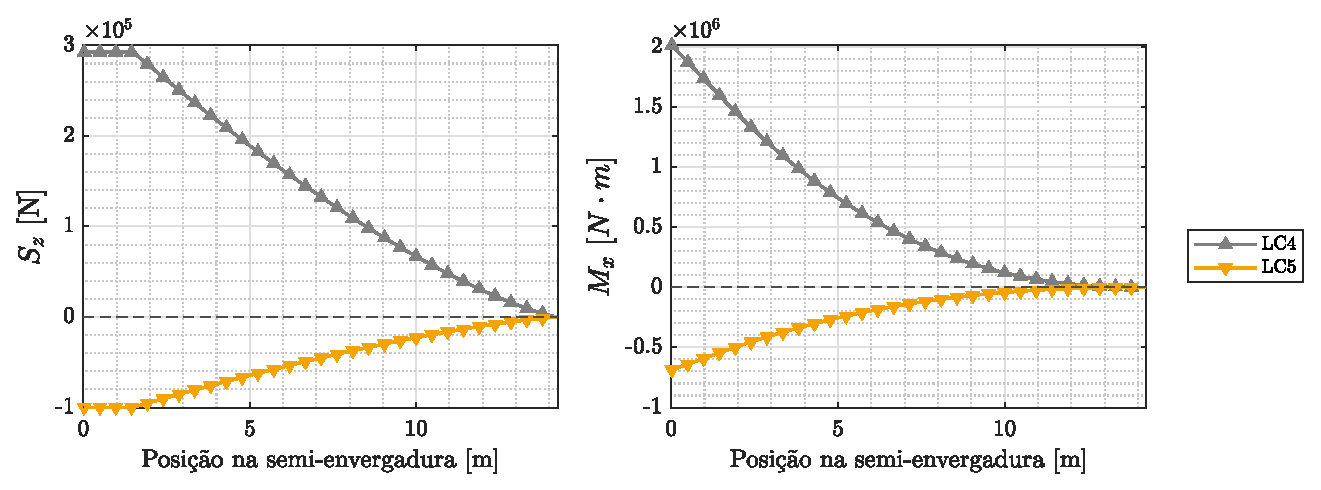
\includegraphics[width=0.91\linewidth]{images/cargas/esforcos_Fz_asa.eps}
    \caption{Esforços críticos associados a $F_z$ na asa.}
    \label{fig:cargas_asa_crit_fz}
\end{figure}

\begin{figure}[H]
    \centering
    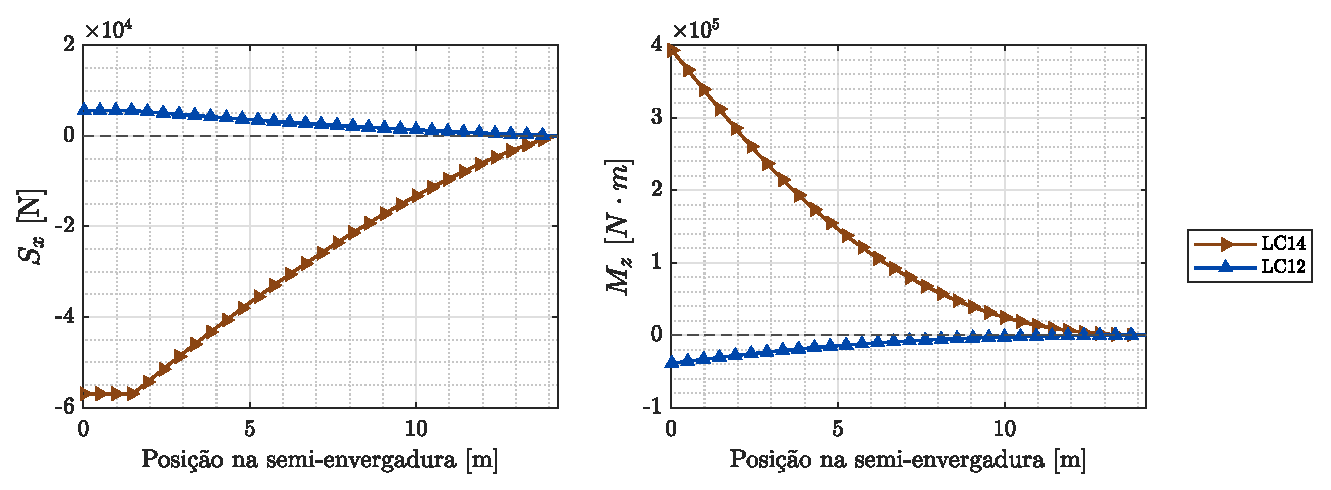
\includegraphics[width=0.91\linewidth]{images/cargas/esforcos_Fx_asa.eps}
    \caption{Esforços críticos associados a $F_x$ na asa.}
    \label{fig:cargas_asa_crit_fx}
\end{figure}

\begin{figure}[H]
    \centering
    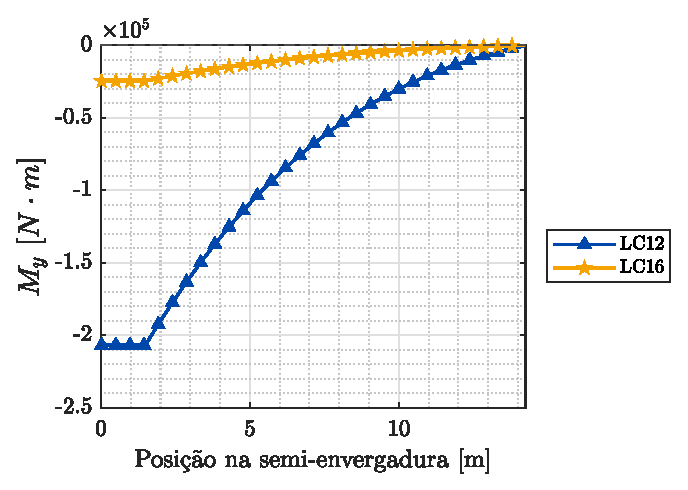
\includegraphics[width=0.55\linewidth]{images/cargas/esforco_MA_asa.eps}
    \caption{Momento torsor crítico $M_y$ na asa.}
    \label{fig:cargas_asa_crit_my}
\end{figure}

\section{Cargas na EH}
\label{sec:cargas_eh}

A análise de cargas da EH considerou as condições de balanceamento, manobra e rajada. Para cada condição, a força aerodinâmica foi determinada e distribuída ao longo da envergadura pelo método de Stender, permitindo o cálculo dos esforços internos correspondentes.

\subsection*{Balanceamento}

As cargas de balanceamento da EH foram determinadas pelo equilíbrio longitudinal apresentado na \autoref{fig:cargas_dcl_balanceamento}, de acordo com
\begin{equation}
    L_t=\frac{\rho_0S_w\bar{c}C_{M_0}}{2\bar{l}_t}V_{\mathrm{EAS}}^2
    +\frac{W(h_{CG}-h_0)\bar{c}}{\bar{l}_t}\,n_z.
    \label{eq:cargas_Lt}
\end{equation}

A Equação~\ref{eq:cargas_Lt} foi aplicada às combinações de velocidade, fator de carga e CG consideradas no envelope.

\subsection*{Manobras}

As cargas de manobra foram estimadas com referência ao \S~25.331 do 14 CFR Part 25. A manobra não corrigida considerou as deflexões máximas positiva e negativa do profundor em $V_A$. Para a manobra corrigida, incluiu-se de forma aproximada o efeito da aceleração angular de arfagem e do momento de inércia longitudinal, como avaliação preliminar do requisito.

\subsection*{Rajada}

As cargas de rajada foram calculadas com referência ao \S~25.341 do 14 CFR Part 25, somando-se à carga de balanceamento em voo a $1\,g$ o incremento aerodinâmico provocado pela rajada:
\begin{equation}
    L_{t,\mathrm{raj}}=L_{t,\mathrm{bal},\,1g}\pm\Delta L_{t,g},
    \label{eq:cargas_Lt_raj}
\end{equation}
\begin{equation}
    \Delta L_{t,g}=\frac{1}{2}\rho_0V_{\mathrm{EAS}}S_ta_tU_gK_g
    \left(1-\frac{\mathrm{d}\varepsilon}{\mathrm{d}\alpha}\right).
    \label{eq:cargas_dLt_raj}
\end{equation}

\subsection*{Arrasto, Momento Aerodinâmico e Distribuição}

De modo semelhante à asa, o arrasto da EH foi estimado com base na sustentação local e nas polares bidimensionais dos perfis utilizados. O momento aerodinâmico foi calculado em relação a $25\%$ da corda local, utilizando as distribuições de carregamento das Figuras B6, B7 e B8 do Apêndice B da CS-VLA, conforme a condição analisada. Essa abordagem, já empregada na metodologia de cargas adotada, foi utilizada como estimativa preliminar, embora a aeronave deste projeto pertença à categoria Transporte.

Os carregamentos das regiões encobertas pela EV foram redistribuídos entre os trechos expostos da EH, preservando-se os valores totais das resultantes. As componentes $F_z$ e $F_x$ foram obtidas pela transformação das forças aerodinâmicas para os eixos da aeronave.

\subsection*{Resultados}

Os carregamentos distribuídos obtidos pelo método de Stender são apresentados na \autoref{fig:cargas_eh_fz}, na \autoref{fig:cargas_eh_fx} e na \autoref{fig:cargas_eh_ma}.

%% Os gráficos de distribuição abaixo abrangem TODAS as condições de carga da EH.
\begin{figure}[H]
    \centering
    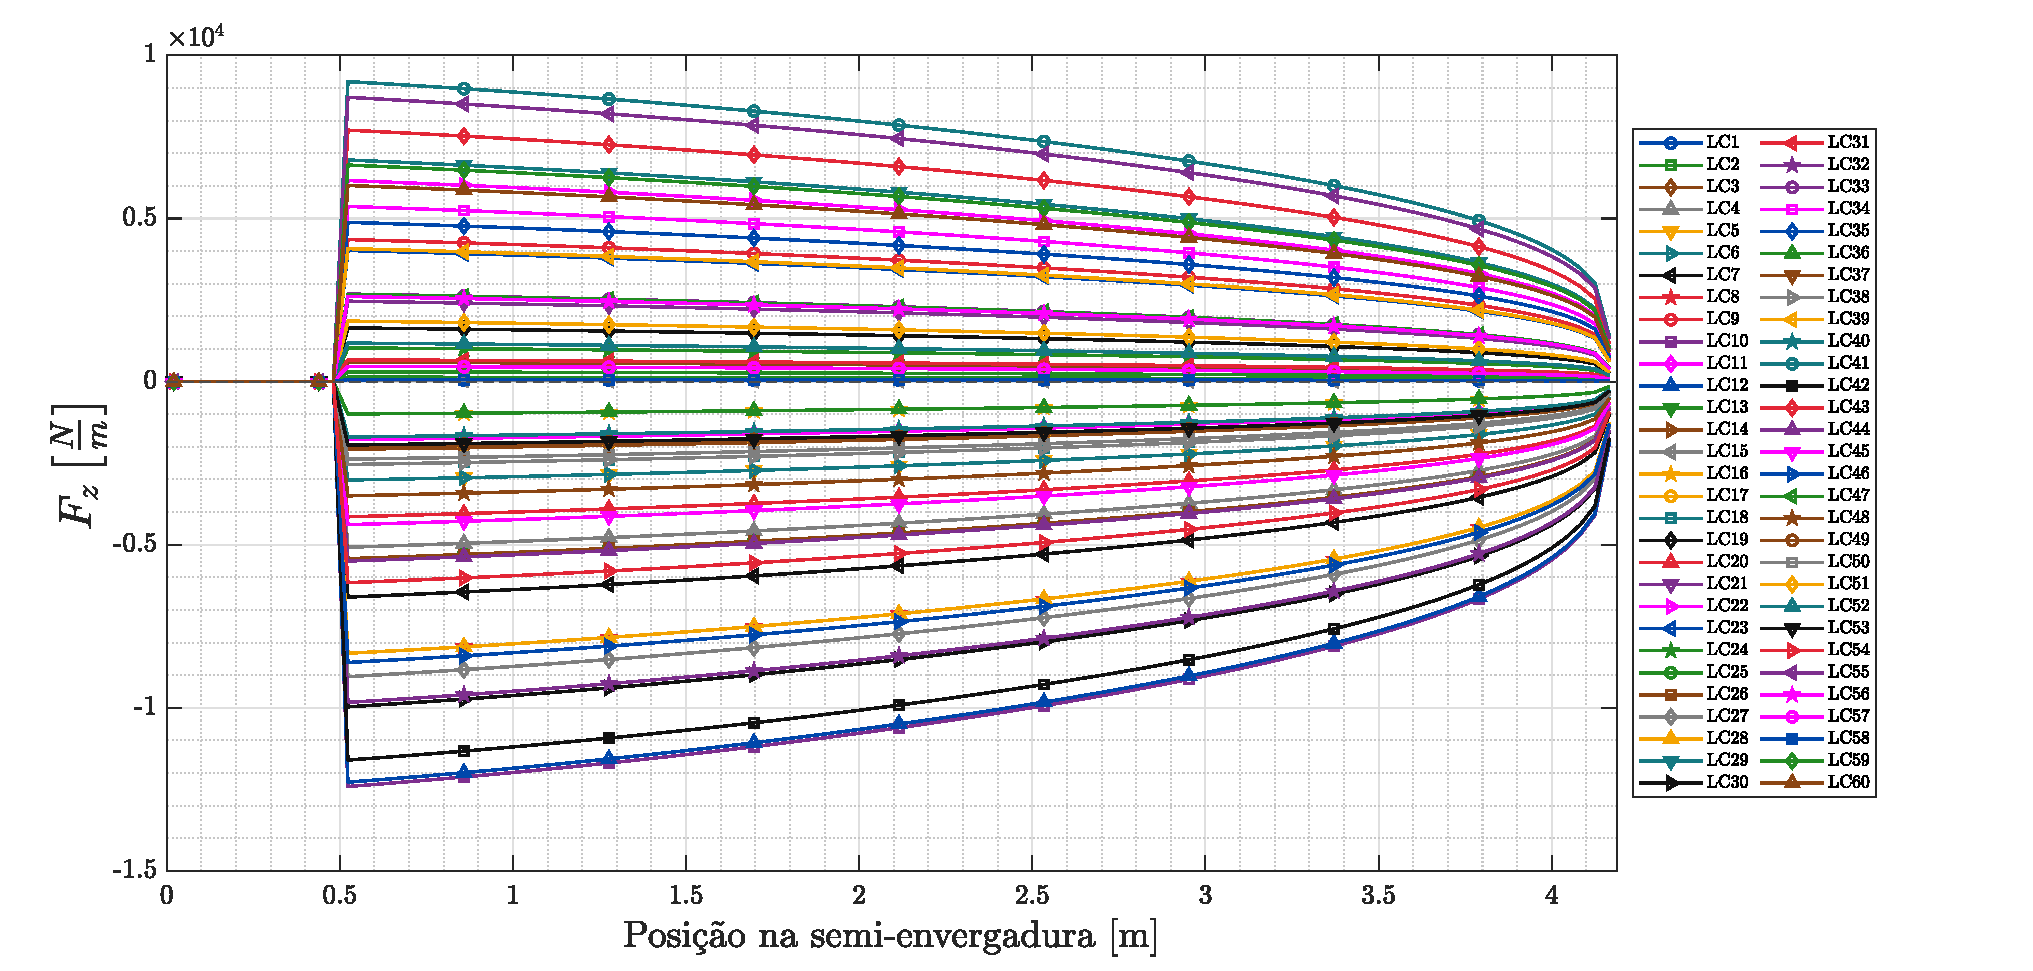
\includegraphics[width=1\linewidth]{images/cargas/htail_Fz.eps}
    \caption{$F_z$ distribuído na EH.}
    \label{fig:cargas_eh_fz}
\end{figure}

\begin{figure}[H]
    \centering
    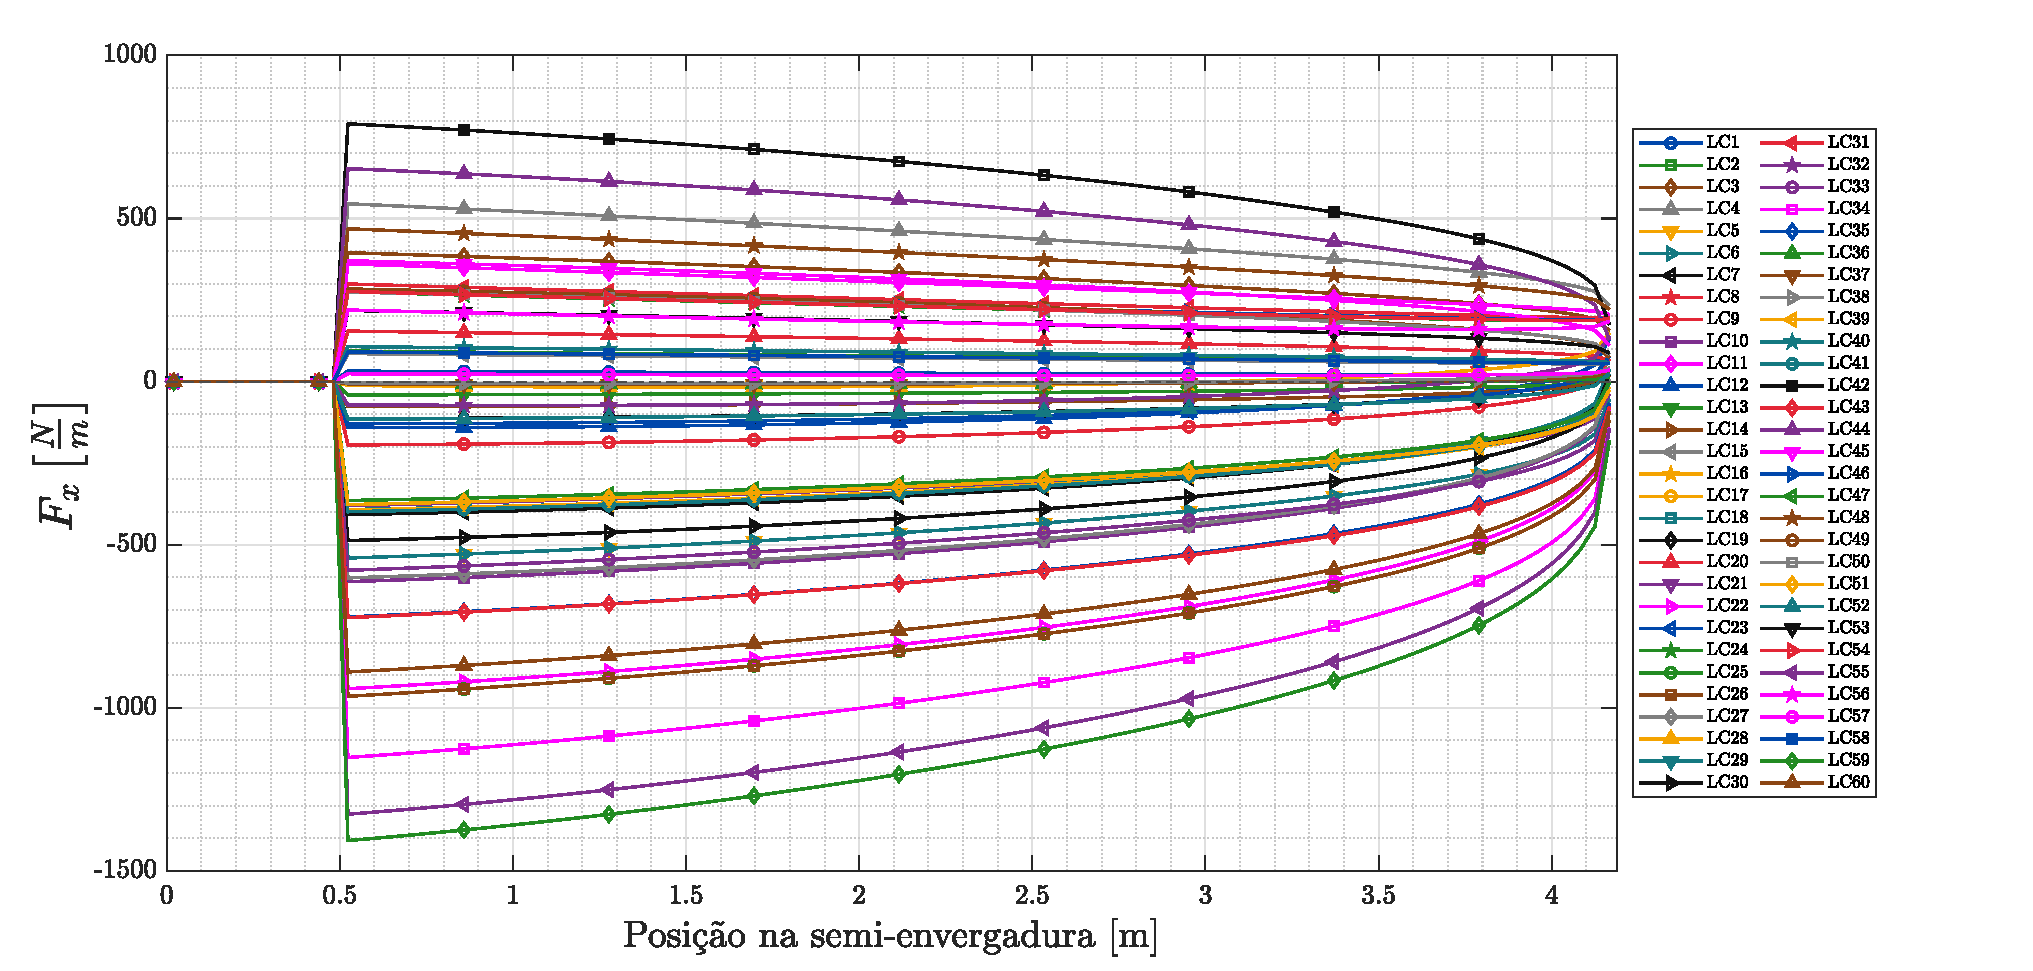
\includegraphics[width=1\linewidth]{images/cargas/htail_Fx.eps}
    \caption{$F_x$ distribuído na EH.}
    \label{fig:cargas_eh_fx}
\end{figure}

\begin{figure}[H]
    \centering
    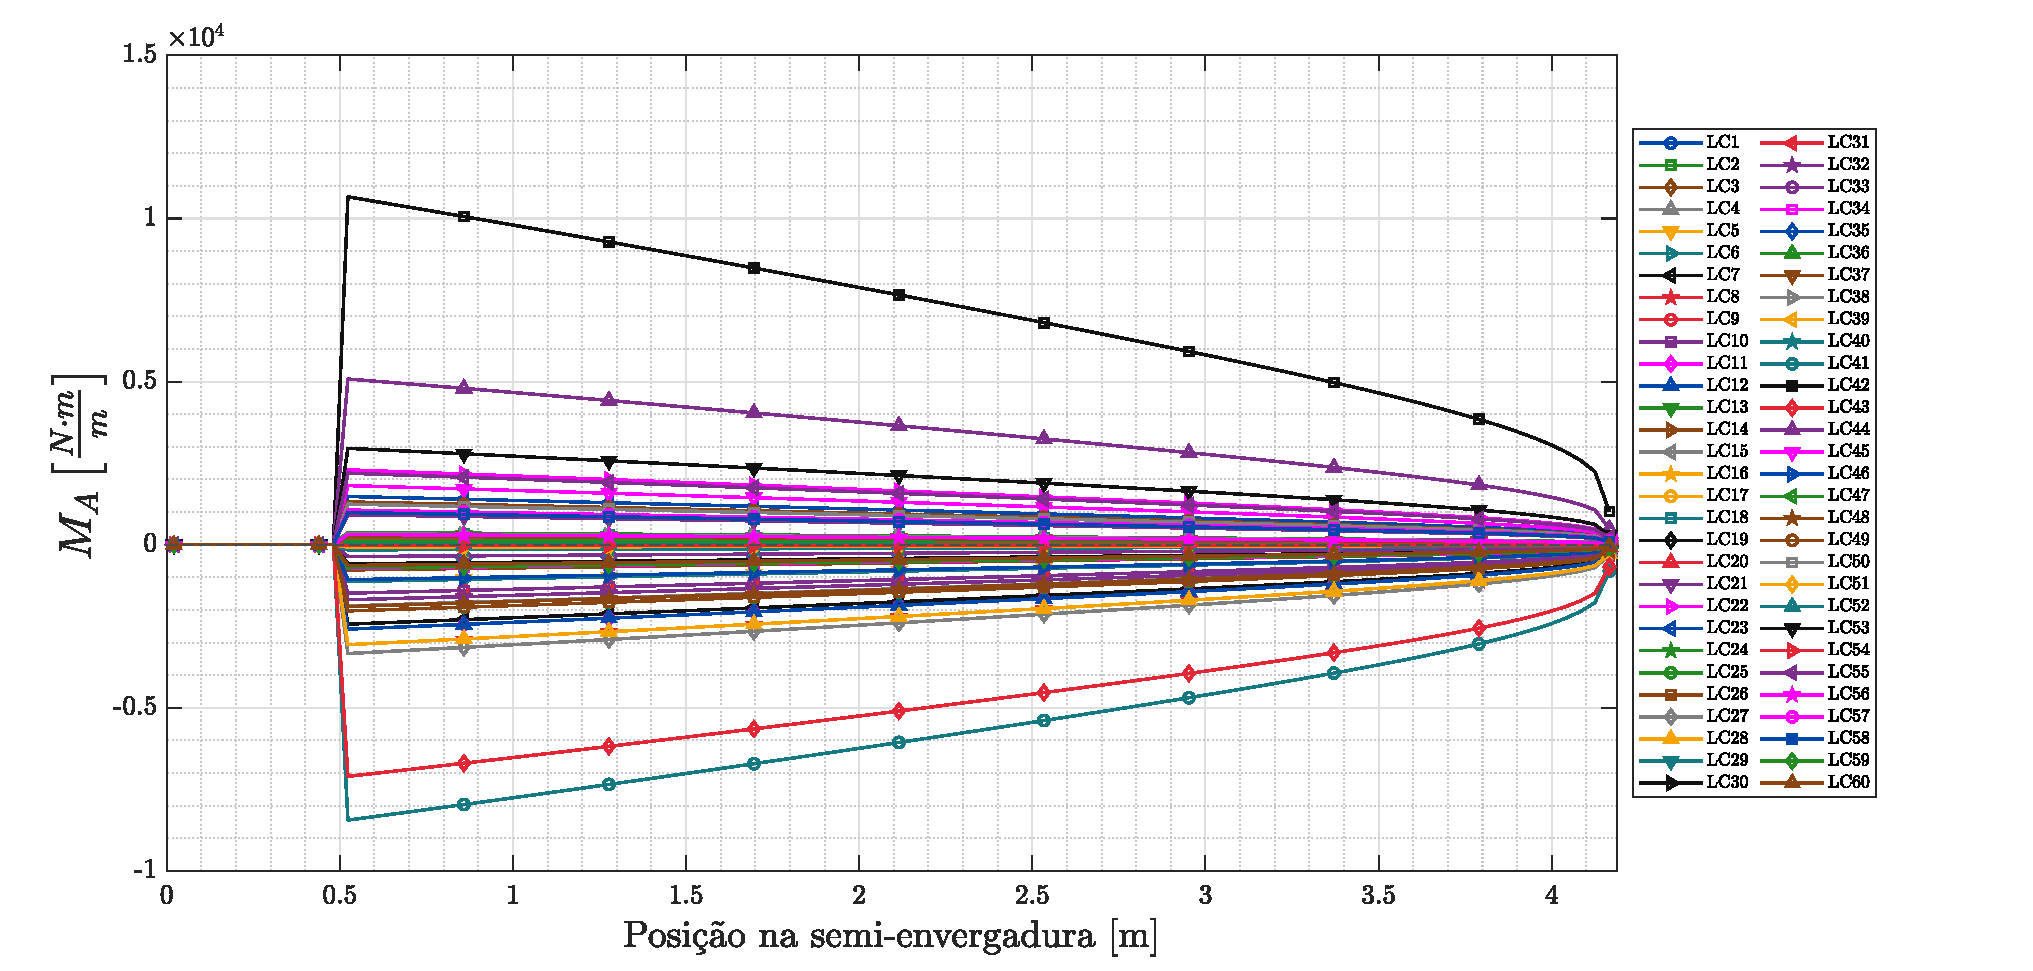
\includegraphics[width=1\linewidth]{images/cargas/htail_MA.eps}
    \caption{$MA$ distribuído na EH.}
    \label{fig:cargas_eh_ma}
\end{figure}

As condições de voo correspondentes aos casos críticos identificados para a EH são resumidas na Tabela~\ref{tab:cargas_criticas_eh}.

\begin{table}[H]
    \centering
    \caption{Condições críticas da EH.}
    \label{tab:cargas_criticas_eh}
    \vspace{1mm}
    \begingroup
    \footnotesize
    \setlength{\tabcolsep}{5pt}
    \renewcommand{\arraystretch}{1.35}
    \begin{tabular}{@{}lccccccc@{}}
        \noalign{\hrule height 0.8pt}
        \textbf{N\textsuperscript{o}} & \textbf{Tipo} & \textbf{14 CFR Part 25} & \textbf{TOW} & \textbf{CG} & \textbf{Flap} & \textbf{Velocidade} & \boldmath$n_z$\\
        \hline
        LC10 & Rajada & \S~25.341 & MTOW & Dianteiro & Recolhido & $V_C$ & $-0{,}32$\\
        LC41 & \shortstack{Manobra não\\corrigida (+)} & \S~25.331 & MTOW & --- & Recolhido & $V_A$ & $1{,}00$\\
        LC42 & \shortstack{Manobra não\\corrigida ($-$)} & \S~25.331 & MTOW & --- & Recolhido & $V_A$ & $1{,}00$\\
        LC59 & \shortstack{Manobra corrigida\\(picada)} & \S~25.331 & MTOW & Traseiro & Estendido & $V_A$ & $2{,}00$\\
        \noalign{\hrule height 0.8pt}
    \end{tabular}
    \endgroup
\end{table}

Os esforços internos correspondentes às condições críticas são apresentados na \autoref{fig:cargas_eh_crit_fz}, na \autoref{fig:cargas_eh_crit_fx} e na \autoref{fig:cargas_eh_crit_my}.

\begin{figure}[H]
    \centering
    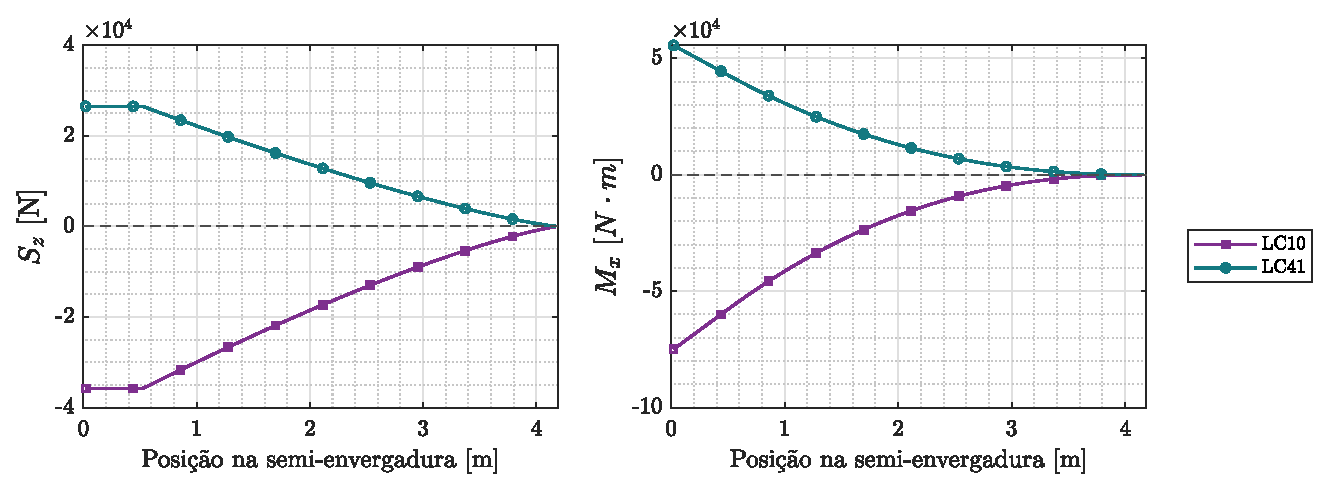
\includegraphics[width=0.91\linewidth]{images/cargas/esforcos_Fz_eh.eps}
    \caption{Esforços críticos associados a $F_z$ na EH.}
    \label{fig:cargas_eh_crit_fz}
\end{figure}

\begin{figure}[H]
    \centering
    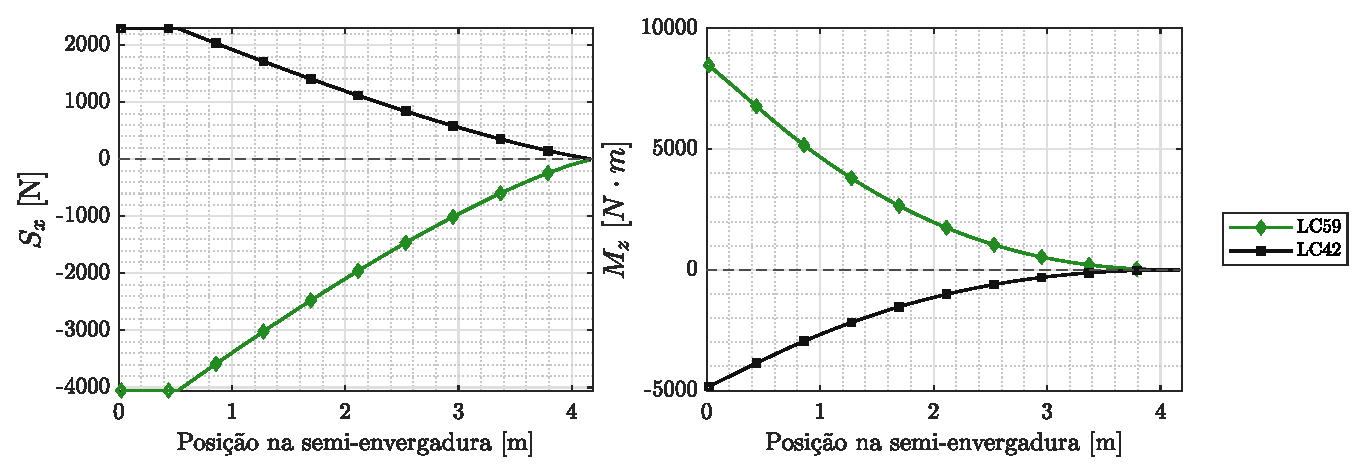
\includegraphics[width=0.91\linewidth]{images/cargas/esforcos_Fx_eh.eps}
    \caption{Esforços críticos associados a $F_x$ na EH.}
    \label{fig:cargas_eh_crit_fx}
\end{figure}

\begin{figure}[H]
    \centering
    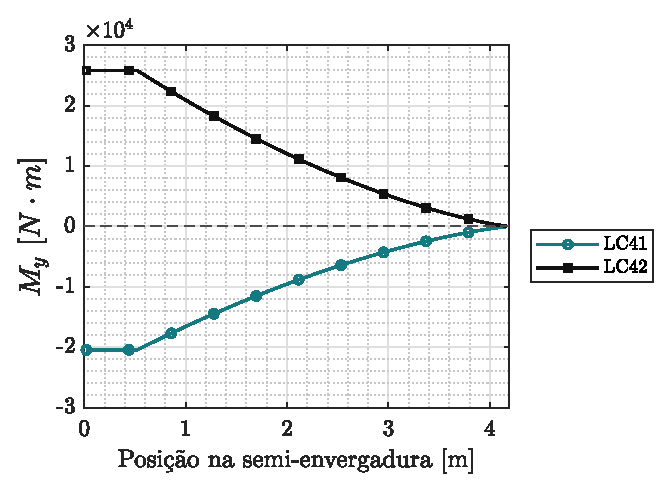
\includegraphics[width=0.55\linewidth]{images/cargas/esforco_MA_eh.eps}
    \caption{Momento torsor crítico $M_y$ na EH.}
    \label{fig:cargas_eh_crit_my}
\end{figure}

\section{Cargas na EV}
\label{sec:cargas_ev}

As cargas da EV foram determinadas para condições de manobra de guinada e rajada lateral. Os carregamentos resultantes foram distribuídos ao longo da altura da EV pelo método de Stender, permitindo a determinação dos esforços internos.

\subsection*{Manobras}

As cargas de manobra foram estimadas com referência ao \S~25.351 do 14 CFR Part 25, considerando a deflexão máxima do leme sem derrapagem e as condições de derrapagem, incluindo o leme neutro. A força lateral foi calculada pela contribuição do ângulo de derrapagem $\beta$ e da deflexão do leme $\zeta$:
\begin{equation}
    C_{L,vt}=a_{vt}\beta+C_{L,vt,\zeta}\zeta,
    \qquad
    L_{vt}=\frac{1}{2}\rho_0V_{\mathrm{EAS}}^2S_{vt}C_{L,vt}.
    \label{eq:cargas_ev_man}
\end{equation}

\subsection*{Rajada}

As cargas de rajada lateral foram estimadas com referência ao \S~25.341 do 14 CFR Part 25, considerando os dois sentidos de incidência da rajada e o fator de alívio adotado no cálculo. O incremento de força lateral foi determinado por
\begin{equation}
    \Delta L_{vt,g}=\frac{1}{2}\rho_0V_{\mathrm{EAS}}S_{vt}
    \left|a_{vt}\right|U_gK_{g,vt}.
    \label{eq:cargas_ev_raj}
\end{equation}

\subsection*{Arrasto, Momento Aerodinâmico e Distribuição}

O arrasto da EV foi estimado a partir da sustentação local e da polar bidimensional do perfil adotado. Para o momento aerodinâmico, utilizou-se a mesma aproximação empregada na EH, com as distribuições das Figuras B6, B7 e B8 do Apêndice B da CS-VLA, referidas a $25\%$ da corda local. Essas distribuições foram adotadas como estimativa preliminar, sem alterar a base normativa de categoria Transporte da aeronave.

As parcelas de força lateral, arrasto e momento aerodinâmico da região não exposta junto à fuselagem foram redistribuídas sobre os trechos externos da EV. As componentes nos eixos da aeronave foram obtidas por
\begin{align}
    F_y &= L_{vt}\cos\beta-D_{vt}\sin\beta, \\
    F_x &= L_{vt}\sin\beta+D_{vt}\cos\beta.
    \label{eq:cargas_transform_ev}
\end{align}

\subsection*{Resultados}

Os carregamentos distribuídos obtidos pelo método de Stender são apresentados na \autoref{fig:cargas_ev_fy}, na \autoref{fig:cargas_ev_fx} e na \autoref{fig:cargas_ev_ma}.

\begin{figure}[H]
    \centering
    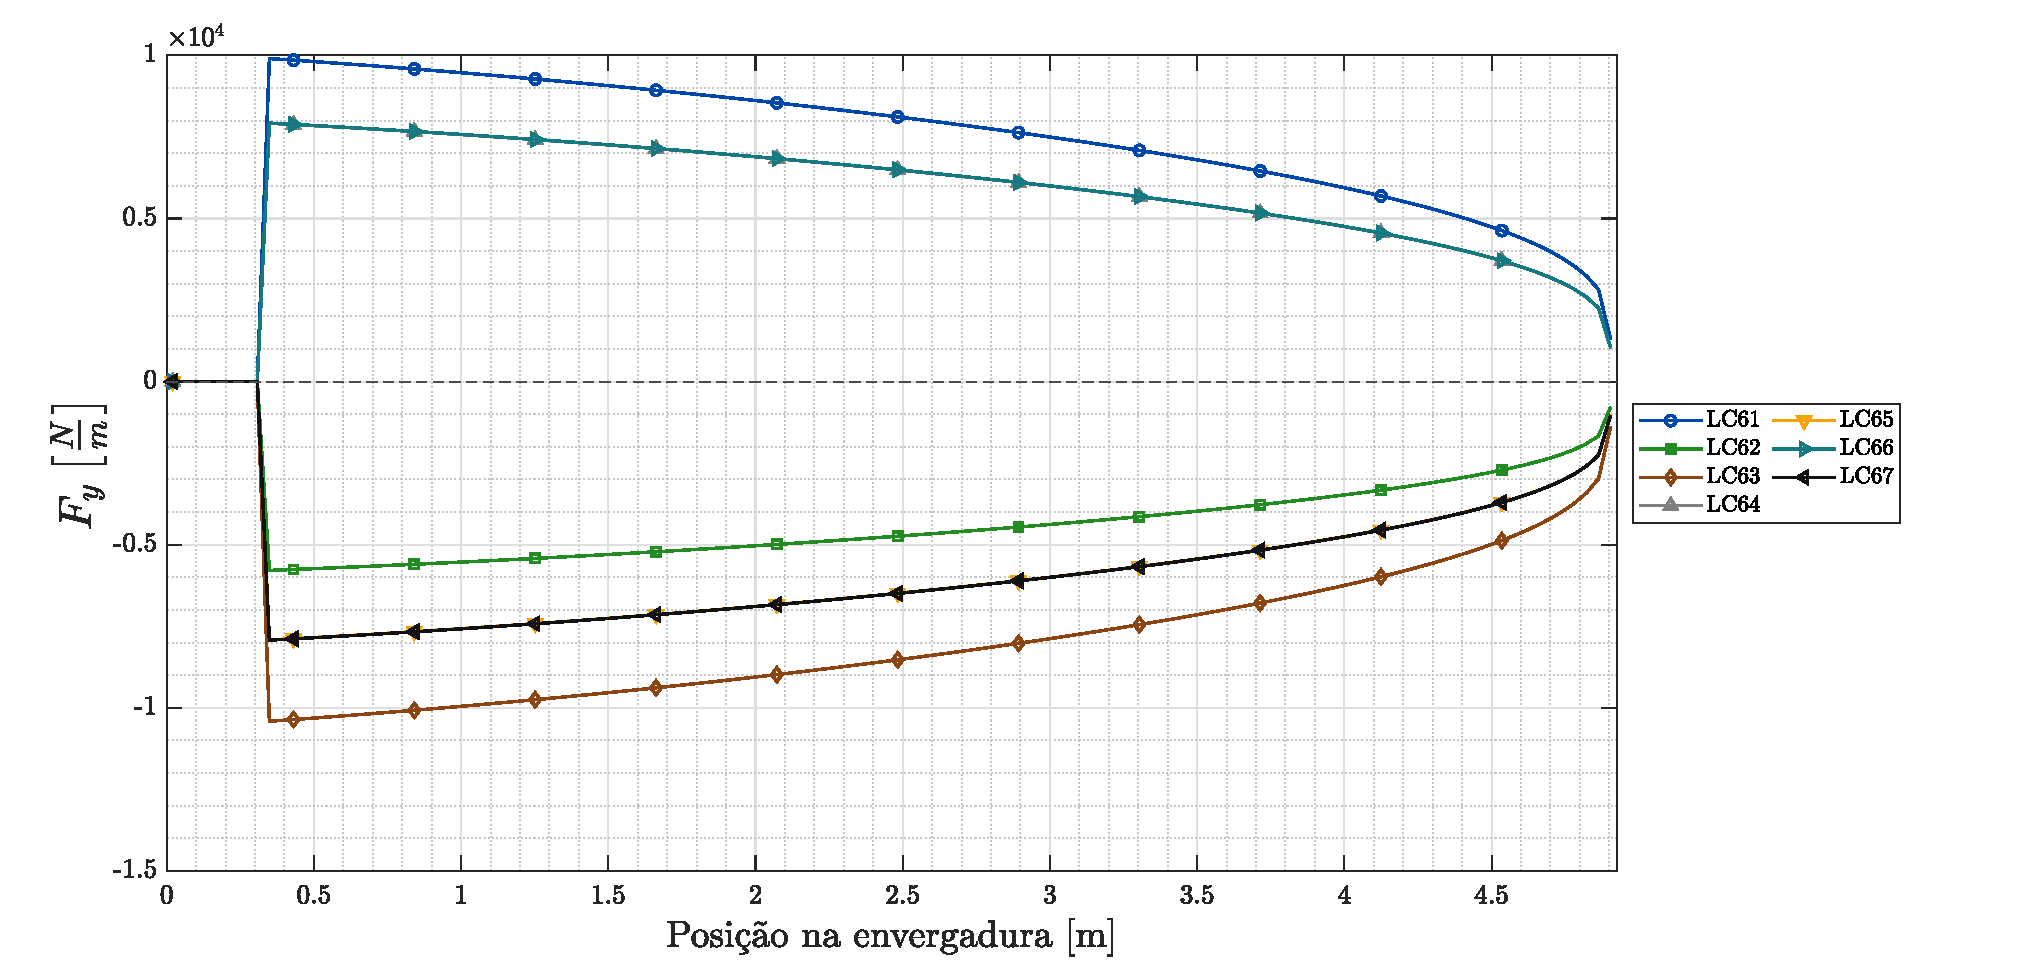
\includegraphics[width=1\linewidth]{images/cargas/vtail_Fy.eps}
    \caption{$F_y$ distribuído na EV.}
    \label{fig:cargas_ev_fy}
\end{figure}

\begin{figure}[H]
    \centering
    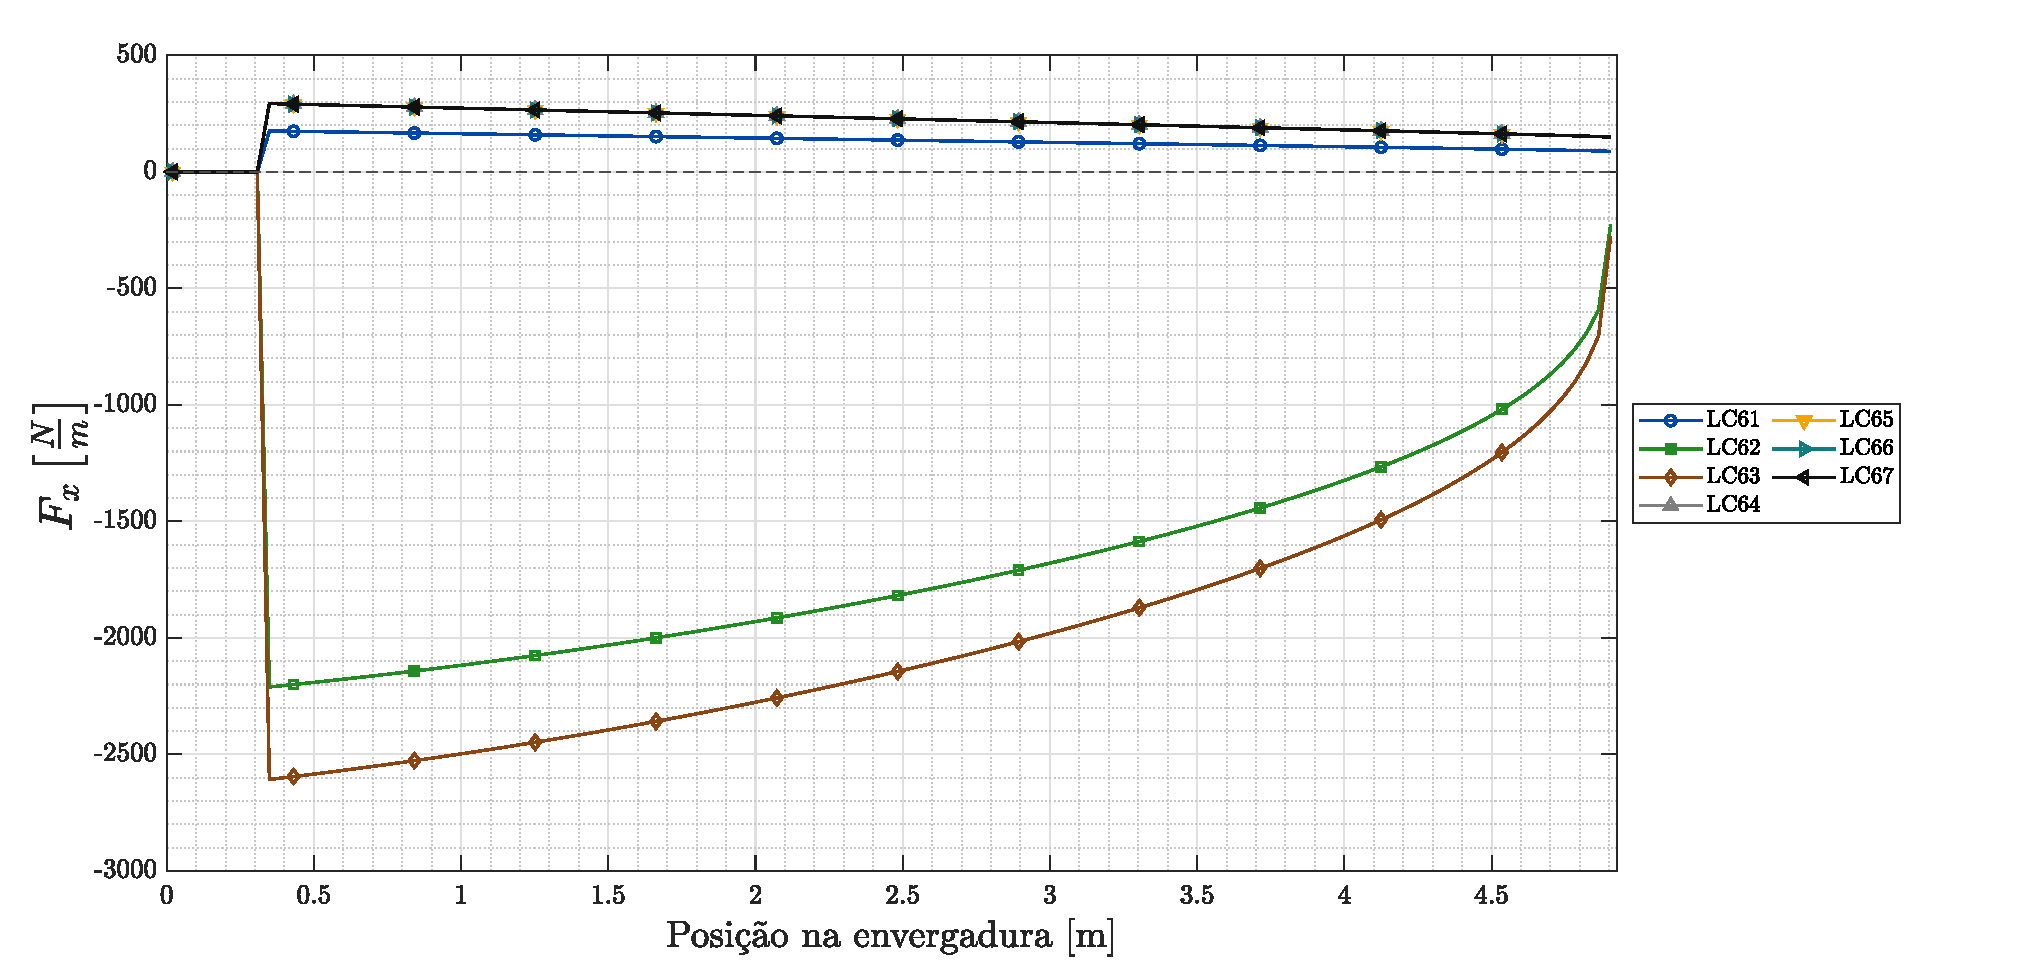
\includegraphics[width=1\linewidth]{images/cargas/vtail_Fx.eps}
    \caption{$F_x$ distribuído na EV.}
    \label{fig:cargas_ev_fx}
\end{figure}

\begin{figure}[H]
    \centering
    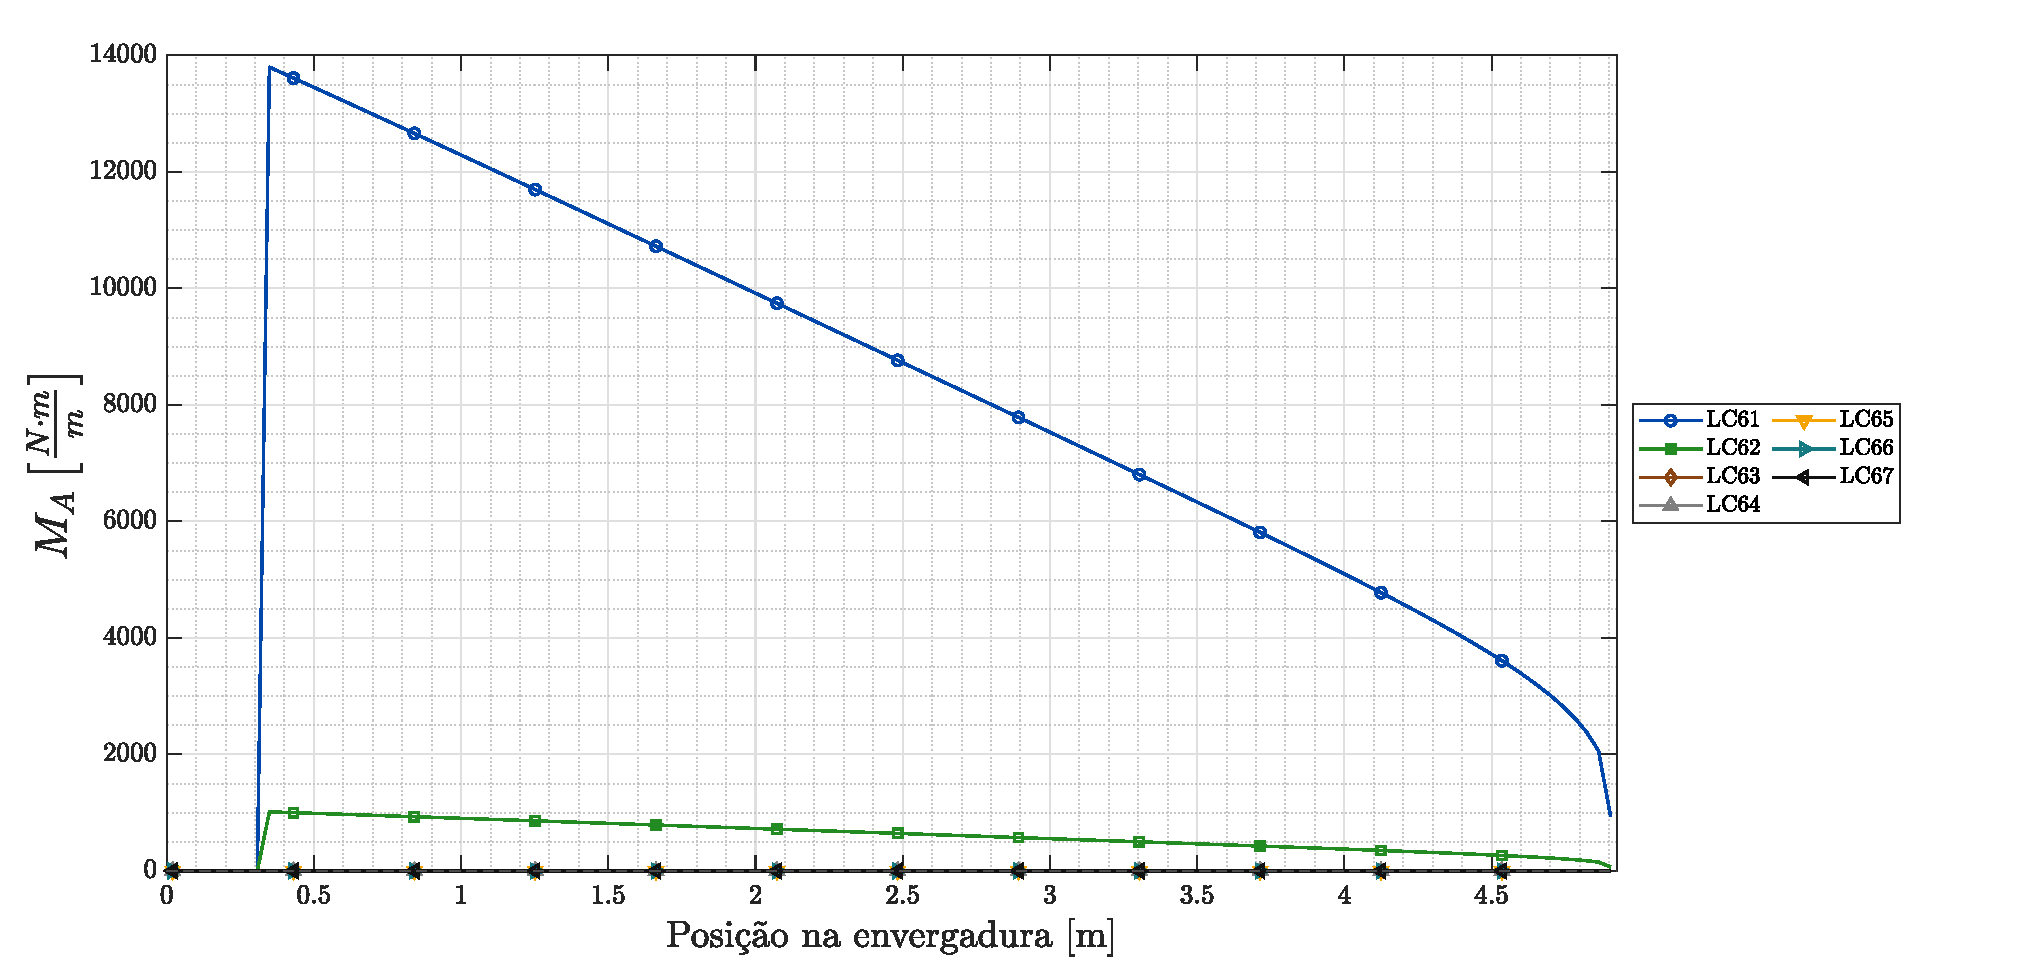
\includegraphics[width=1\linewidth]{images/cargas/vtail_MA.eps}
    \caption{$MA$ distribuído na EV.}
    \label{fig:cargas_ev_ma}
\end{figure}

As condições de voo correspondentes aos casos críticos identificados para a EV são resumidas na Tabela~\ref{tab:cargas_criticas_ev}.

\begin{table}[H]
    \centering
    \caption{Condições críticas da EV.}
    \label{tab:cargas_criticas_ev}
    \vspace{1mm}
    \begingroup
    \footnotesize
    \setlength{\tabcolsep}{5pt}
    \renewcommand{\arraystretch}{1.35}
    \begin{tabular}{@{}lccccccc@{}}
        \noalign{\hrule height 0.8pt}
        \textbf{N\textsuperscript{o}} & \textbf{Tipo} & \textbf{14 CFR Part 25} & \textbf{TOW} & \textbf{CG} & \textbf{Flap} & \textbf{Velocidade} & \textbf{Condição}\\
        \hline
        LC61 & Manobra & \S~25.351 & MTOW & --- & Recolhido & $V_A$ & $\zeta=+30^\circ$\\
        LC63 & Manobra & \S~25.351 & MTOW & --- & Recolhido & $V_A$ & $\beta=15^\circ$\\
        LC66 & Rajada & \S~25.341 & MTOW & Traseiro & Recolhido & $V_C$ & Rajada (+)\\
        \noalign{\hrule height 0.8pt}
    \end{tabular}
    \endgroup
\end{table}

Os esforços internos correspondentes às condições críticas são apresentados na \autoref{fig:cargas_ev_crit_fy}, na \autoref{fig:cargas_ev_crit_fx} e na \autoref{fig:cargas_ev_crit_mz}.

%% Os gráficos de esforços abaixo incluem SOMENTE as condições críticas.
\begin{figure}[H]
    \centering
    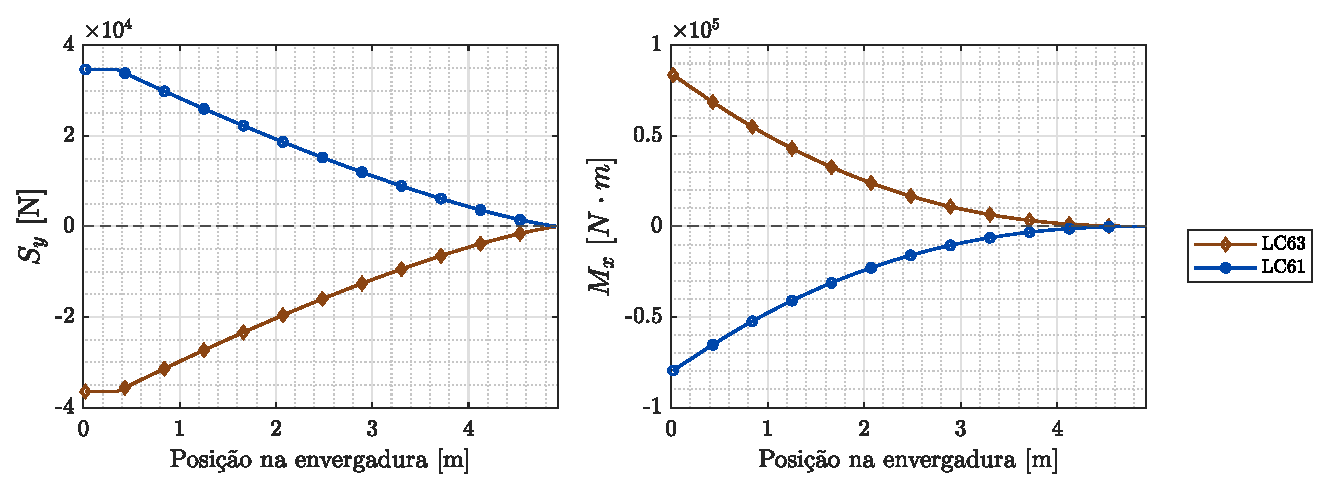
\includegraphics[width=0.91\linewidth]{images/cargas/esforcos_Fy_ev.eps}
    \caption{Esforços críticos associados a $F_y$ na EV.}
    \label{fig:cargas_ev_crit_fy}
\end{figure}

\begin{figure}[H]
    \centering
    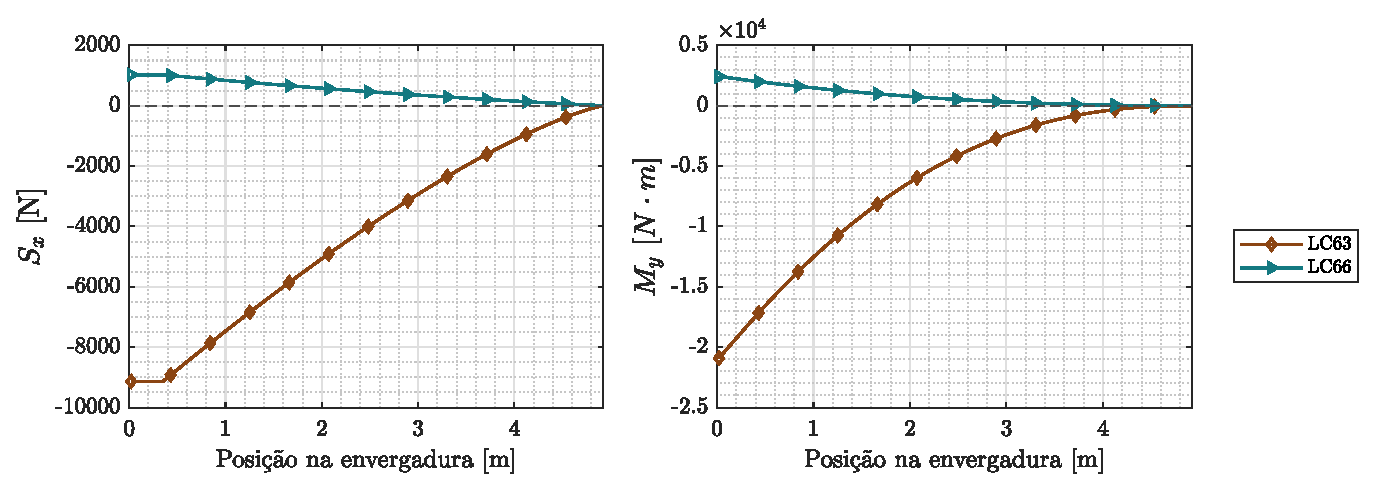
\includegraphics[width=0.91\linewidth]{images/cargas/esforcos_Fx_ev.eps}
    \caption{Esforços críticos associados a $F_x$ na EV.}
    \label{fig:cargas_ev_crit_fx}
\end{figure}

\begin{figure}[H]
    \centering
    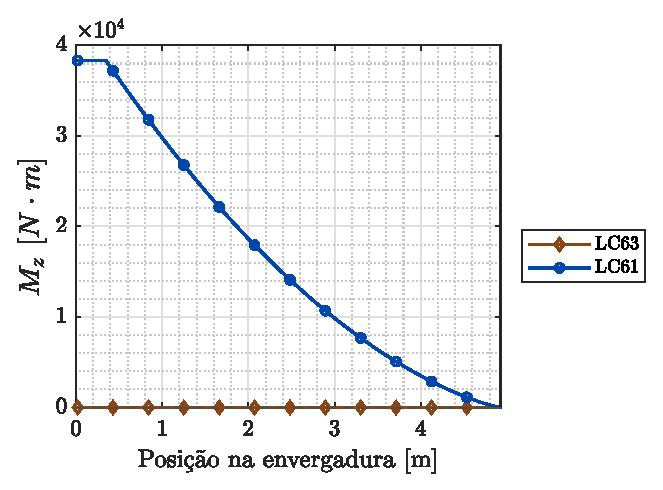
\includegraphics[width=0.55\linewidth]{images/cargas/esforco_MA_ev.eps}
    \caption{Momento torsor crítico $M_z$ na EV.}
    \label{fig:cargas_ev_crit_mz}
\end{figure}

Vale ressaltar que as manobras da empenagem vertical são simétricas em relação ao plano longitudinal da aeronave. Dessa forma, os casos foram avaliados em apenas um sentido, sendo o envelope de cargas considerado equivalente para o sentido oposto.

\section{Cargas no Trem de Pouso}
\label{sec:cargas_solo}


A determinação das cargas atuantes no trem de pouso durante as operações de toque e rolagem foi realizada considerando cinco condições críticas de pouso. De modo análogo às simplificações preliminares adotadas nas seções anteriores para as empenagens, recorreu-se à metodologia analítica simplificada prescrita nas seções \S 23.479 a \S 23.485 e no Apêndice C do 14 CFR Part 23 (correspondentes às condições equivalentes das seções \S 25.479 a \S 25.485 do 14 CFR Part 25 e RBAC 25). Essa abordagem permite estimar as reações estáticas equivalentes nas pernas do trem de pouso principal (TDPP) e do trem de pouso auxiliar de nariz (TDPA) sem exigir, nesta fase do projeto preliminar, a modelagem dinâmica não-linear dos amortecedores óleo-pneumáticos, mantendo-se inalterada a base certificadora da aeronave na Categoria Transporte.

\subsubsection*{Sistema de Coordenadas e Parâmetros de Entrada}

% A geometria das pernas do trem de pouso é referenciada ao Centro de Gravidade (CG) da aeronave no sistema de eixos de corpo, no qual o eixo $+x_b$ aponta para a frente, $+y_b$ para a semiasa direita e $+z_b$ verticalmente para baixo. As coordenadas do ponto de contato de cada conjunto com o solo em relação ao CG são definidas pelos vetores posição $\vec{r}_{\text{TDPP}} = [x_m, \, y_m, \, z_m]$ e $\vec{r}_{\text{TDPA}} = [x_n, \, 0, \, z_n]$.

% Por sua vez, as reações de contato provenientes do solo sobre os pneus são expressas no referencial de cargas de saída, adotando-se o eixo $+X$ orientado longitudinalmente para trás (sentido da força de arrasto de \textit{spin-up} das rodas), $+Y$ lateralmente para a direita e $+Z$ verticalmente para cima (reação normal à pista).

% Os cálculos foram conduzidos para a condição crítica de Peso Máximo de Decolagem ($\text{MTOW} = 22\,680\text{ kg}$, correspondente a $W = \text{MTOW} \cdot g$).
Adotou-se um fator de carga inercial limite vertical no CG igual a $n_{\text{inertia}} = 2,67$ e uma fração máxima de sustentação aerodinâmica remanescente no instante do toque de $k_L = L/W = 2/3$. Dessa forma, o fator de carga vertical líquido transmitido ao solo ($n_{\text{ground}}$) nas condições simétricas de impacto é dado por:
\begin{equation}
    n_{\text{ground}} = n_{\text{inertia}} - k_L = 2,00.
    \label{eq:n_ground}
\end{equation}

Adicionalmente, a razão entre a componente longitudinal de arrasto e a reação vertical ($D/V$) decorrente da aceleração rotacional das rodas no toque é $K = 0,33$ do Apêndice C da norma, resultando em:
\begin{equation}
    r_{DV} = \frac{K \, n_{\text{inertia}}}{n_{\text{ground}}}.
    \label{eq:r_dv}
\end{equation}

\subsubsection*{Condições de Carregamento Avaliadas}

A seguir, detalham-se as hipóteses físicas e as equações de equilíbrio estático aplicadas a cada um dos cinco casos de carga (\textit{Load Cases}) implementados computacionalmente:

\begin{itemize}
    \item \textbf{Condição C1 -- Pouso em três rodas:} Considera a aeronave em atitude nivelada com toque simultâneo dos trens principal e de nariz.
    \begin{equation}
        F_{z,\text{TDPA}} = W \, n_{\text{ground}} \, \frac{-x_m + r_{DV} \, z_n}{x_n - x_m},
        \label{eq:c1_nose_z}
    \end{equation}
    \begin{equation}
        F_{z,\text{TDPP1}} = F_{z,\text{TDPP2}} = \frac{1}{2} \, W \, n_{\text{ground}} \, \frac{x_n - r_{DV} \, z_m}{x_n - x_m}.
        \label{eq:c1_main_z}
    \end{equation}
    As componentes longitudinais atuantes em cada perna são proporcionais às respectivas cargas normais ($F_x = r_{DV} \, F_z$), totalizando uma força longitudinal de arrasto $D_{\text{tot}} = K \, n_{\text{inertia}} \, W$, enquanto as componentes laterais são nulas ($F_y = 0$).

    \item \textbf{Condição C2 -- Pouso em duas rodas nivelado :} A aeronave encontra-se em atitude longitudinal nivelada, porém o contato ocorre exclusivamente pelas duas pernas do trem de pouso principal ($\vec{F}_{\text{TDPA}} = \vec{0}$).
    \begin{equation}
        F_{z,\text{TDPP1}} = F_{z,\text{TDPP2}} = \frac{1}{2} \, n_{\text{ground}} \, W, \qquad F_{x,\text{TDPP1}} = F_{x,\text{TDPP2}} = r_{DV} \, F_{z,\text{TDPP1}}.
        \label{eq:c2_loads}
    \end{equation}

    \item \textbf{Condição C3 -- Pouso em duas rodas com cauda abaixada :} Representa o toque na atitude de máximo ângulo de ataque (estol ou próximo ao estol), com contato restrito às rodas principais ($\vec{F}_{\text{TDPA}} = \vec{0}$). Nessa configuração geométrica, a resultante de impacto atua na direção vertical pura, de modo que as componentes longitudinais e laterais são nulas:
    \begin{equation}
        F_{z,\text{TDPP1}} = F_{z,\text{TDPP2}} = \frac{1}{2} \, n_{\text{ground}} \, W, \qquad F_{x} = F_{y} = 0.
        \label{eq:c3_loads}
    \end{equation}

    \item \textbf{Condição C4 -- Pouso em uma roda :} Simula uma aterrissagem assimétrica com inclinação lateral, na qual apenas uma das pernas do trem principal (adotada como TDPP1, lado direito) toca a pista, enquanto a perna oposta e o trem de nariz permanecem livres ($\vec{F}_{\text{TDPP2}} = \vec{F}_{\text{TDPA}} = \vec{0}$).
    \begin{equation}
        F_{z,\text{TDPP1}} = \frac{1}{2} \, n_{\text{ground}} \, W, \qquad F_{x,\text{TDPP1}} = r_{DV} \, F_{z,\text{TDPP1}}, \qquad F_{y,\text{TDPP1}} = 0.
        \label{eq:c4_loads}
    \end{equation}

    \item \textbf{Condição C5 -- Pouso em duas rodas com carga lateral:} Avalia o toque em atitude nivelada sob efeito de derrapagem.
    \begin{equation}
        F_{z,\text{TDPP1}} = F_{z,\text{TDPP2}} = \frac{1}{2} \, n_{g,\text{side}} \, W,
        \label{eq:c5_z}
    \end{equation}
    \begin{equation}
        F_{y,\text{TDPP1}} = -0,50 \, W, \qquad F_{y,\text{TDPP2}} = -0,33 \, W.
        \label{eq:c5_y}
    \end{equation}
\end{itemize}

\subsubsection*{Resultados}

As componentes de força nos eixos $X$, $Y$ e $Z$ obtidas para o Trem de Pouso Principal direito (TDPP1), Trem de Pouso Principal esquerdo (TDPP2) e Trem de Pouso Auxiliar de nariz (TDPA) em cada uma das cinco condições analisadas encontram-se consolidadas na Tabela~\ref{tab:cargas_pouso}.

\begin{table}[H]
\centering
\caption{Cargas limite atuantes no trem de pouso por condição de operação.}
\label{tab:cargas_pouso}
\setlength{\tabcolsep}{4.5pt}
\renewcommand{\arraystretch}{1.2}
\resizebox{\textwidth}{!}{%
\begin{tabular}{c l r r r r r r r r r}
\hline
\textbf{Cond.} & \textbf{Descrição} & \multicolumn{3}{c}{\textbf{TDPP 1 (Dir.) [kN]}} & \multicolumn{3}{c}{\textbf{TDPP 2 (Esq.) [kN]}} & \multicolumn{3}{c}{\textbf{TDPA (Nariz) [kN]}} \\
 & & \multicolumn{1}{c}{$F_x$} & \multicolumn{1}{c}{$F_y$} & \multicolumn{1}{c}{$F_z$} & \multicolumn{1}{c}{$F_x$} & \multicolumn{1}{c}{$F_y$} & \multicolumn{1}{c}{$F_z$} & \multicolumn{1}{c}{$F_x$} & \multicolumn{1}{c}{$F_y$} & \multicolumn{1}{c}{$F_z$} \\
\hline
\textbf{C1} & Pouso em três rodas & 91,53 & 0,00 & 207,90 & 91,53 & 0,00 & 207,90 & 13,01 & 0,00 & 29,54 \\
\textbf{C2} & Pouso em duas rodas nivelado & 97,80 & 0,00 & 222,14 & 97,80 & 0,00 & 222,14 & 0,00 & 0,00 & 0,00 \\
\textbf{C3} & Pouso em duas rodas cauda abaixada & 0,00 & 0,00 & 222,14 & 0,00 & 0,00 & 222,14 & 0,00 & 0,00 & 0,00 \\
\textbf{C4} & Pouso em uma roda & 97,80 & 0,00 & 222,14 & 0,00 & 0,00 & 0,00 & 0,00 & 0,00 & 0,00 \\
\textbf{C5} & Pouso em duas rodas com carga lateral & 0,00 & -111,21 & 147,91 & 0,00 & -73,40 & 147,91 & 0,00 & 0,00 & 0,00 \\
\hline
\end{tabular}%
}
\end{table}

A análise da Tabela~\ref{tab:cargas_pouso} evidencia que a solicitação vertical máxima no trem de pouso principal ocorre nas condições C2, C3 e C4, atingindo uma reação normal de $222\,136,52\text{ N}$ por perna, acompanhada de uma força longitudinal máxima de arrasto (\textit{spin-up}) de $97\,798,37\text{ N}$ nas condições C2 e C4. No que tange aos esforços laterais, a Condição C5 impõe o carregamento crítico de derrapagem, resultando em forças de $-111\,207,41\text{ N}$ na perna direita (TDPP1) e $-73\,396,89\text{ N}$ na perna esquerda (TDPP2). Por sua vez, o trem de pouso auxiliar de nariz (TDPA) atinge seu carregamento dimensionante na Condição C1 (pouso nivelado em três rodas), suportando uma carga limite vertical de $29\,541,51\text{ N}$ e longitudinal de $13\,006,07\text{ N}$.